\documentclass[aspectratio=169, 8pt, xcolor={svgnames}, hyperref={linkcolor=black}]{beamer}
\usetheme[progressbar=frametitle]{metropolis}
\setbeamercolor{background canvas}{bg=white}
\setbeamerfont{footnote}{size=\tiny}
\usepackage{appendixnumberbeamer}
\usepackage{url}
\usepackage{amsfonts} 
\usepackage{amssymb}
\usepackage[english]{babel}
\usepackage{fontawesome}
\usepackage{multicol}
\usepackage{bm}
\usepackage{braket}
\usepackage{algorithm}
\usepackage{algpseudocode}
\usepackage{enumitem}

\usepackage[]{pseudo}

\usepackage{tikz}
\usetikzlibrary{positioning,arrows,calc,math,angles,quotes}
\usepackage{blochsphere}

\usetikzlibrary{arrows,automata}
\usetikzlibrary{positioning}
\usetikzlibrary{arrows.meta,
                bending,
                intersections,
                quotes,
                shapes.geometric}

\tikzset{
    state/.style={
           rectangle,
           rounded corners,
           draw=black, very thick,
           minimum height=1em,
           inner sep=2pt,
           text centered,
           },
}

\definecolor{myv}{rgb}{0.36, 0.22, 0.33}
\definecolor{gio}{rgb}{0.45, 0.31, 0.59}
\definecolor{light}{rgb}{0.8, 0.8, 1}
\definecolor{warmblack}{rgb}{0.0, 0.26, 0.26}
\definecolor{brown(web)}{rgb}{0.65, 0.16, 0.16}
\definecolor{cadmiumgreen}{rgb}{0.0, 0.42, 0.24}
\definecolor{darkmidnightblue}{rgb}{0.0, 0.2, 0.4}
\definecolor{brightube}{rgb}{0.82, 0.62, 0.91}
\definecolor{bleudefrance}{rgb}{0.19, 0.55, 0.91}
\definecolor{brightmaroon}{rgb}{0.76, 0.13, 0.28}
\definecolor{codegreen}{rgb}{0,0.6,0}
\definecolor{codegray}{rgb}{0.5,0.5,0.5}
\definecolor{codepurple}{rgb}{0.58,0,0.82}
\definecolor{backcolour}{rgb}{0.95,0.95,0.92}
\definecolor{amethyst}{rgb}{0.6, 0.33, 0.73}

\usepackage[most]{tcolorbox}
\usepackage{xcolor}


\title{Quantum Machine Learning in HEP with \texttt{Qibo}}
\subtitle{PyHEP 2024}
\date{3 July 2023}
\author{Matteo Robbiati$^\dagger$ on behalf of the Qibo team$^\ddag$}
\institute{$^\dagger$ PhD candidate, University of Milan, Italy and CERN, Switzerland. \\\faEnvelope~\texttt{matteo.robbiati@cern.ch} 
\\ \\ $^\ddag \href{https://qibo.science/}{https://qibo.science/}$}
\titlegraphic{
   \begin{tikzpicture}[overlay, remember picture]
   \node[at=(current page.south east), anchor=south east] {%
      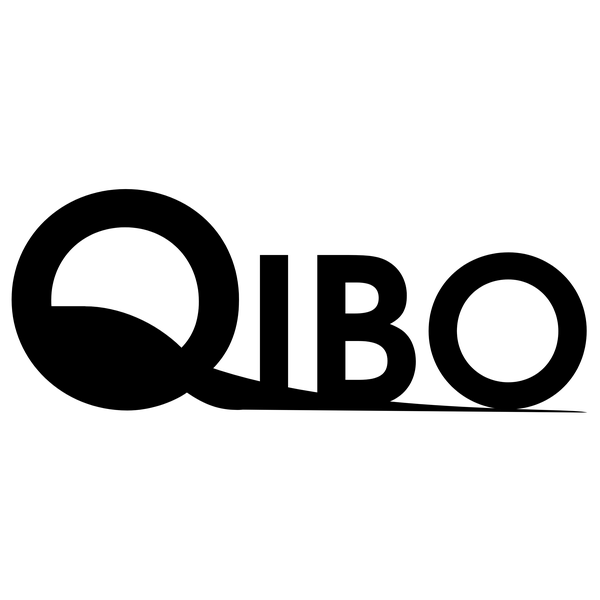
\includegraphics[width=.15\textwidth]{figures/qibo.png} 
      
\includegraphics[width=.15\textwidth]{figures/unimi.png} 
      
\includegraphics[width=.15\textwidth]{figures/cern.png}  
      
\includegraphics[width=.15\textwidth]{figures/qti.png}  
   };
   \end{tikzpicture}
}

\begin{document}

\begin{frame}
\maketitle
\end{frame}

\begin{frame}{Quantum Computing for HEP}
\begin{figure}  
    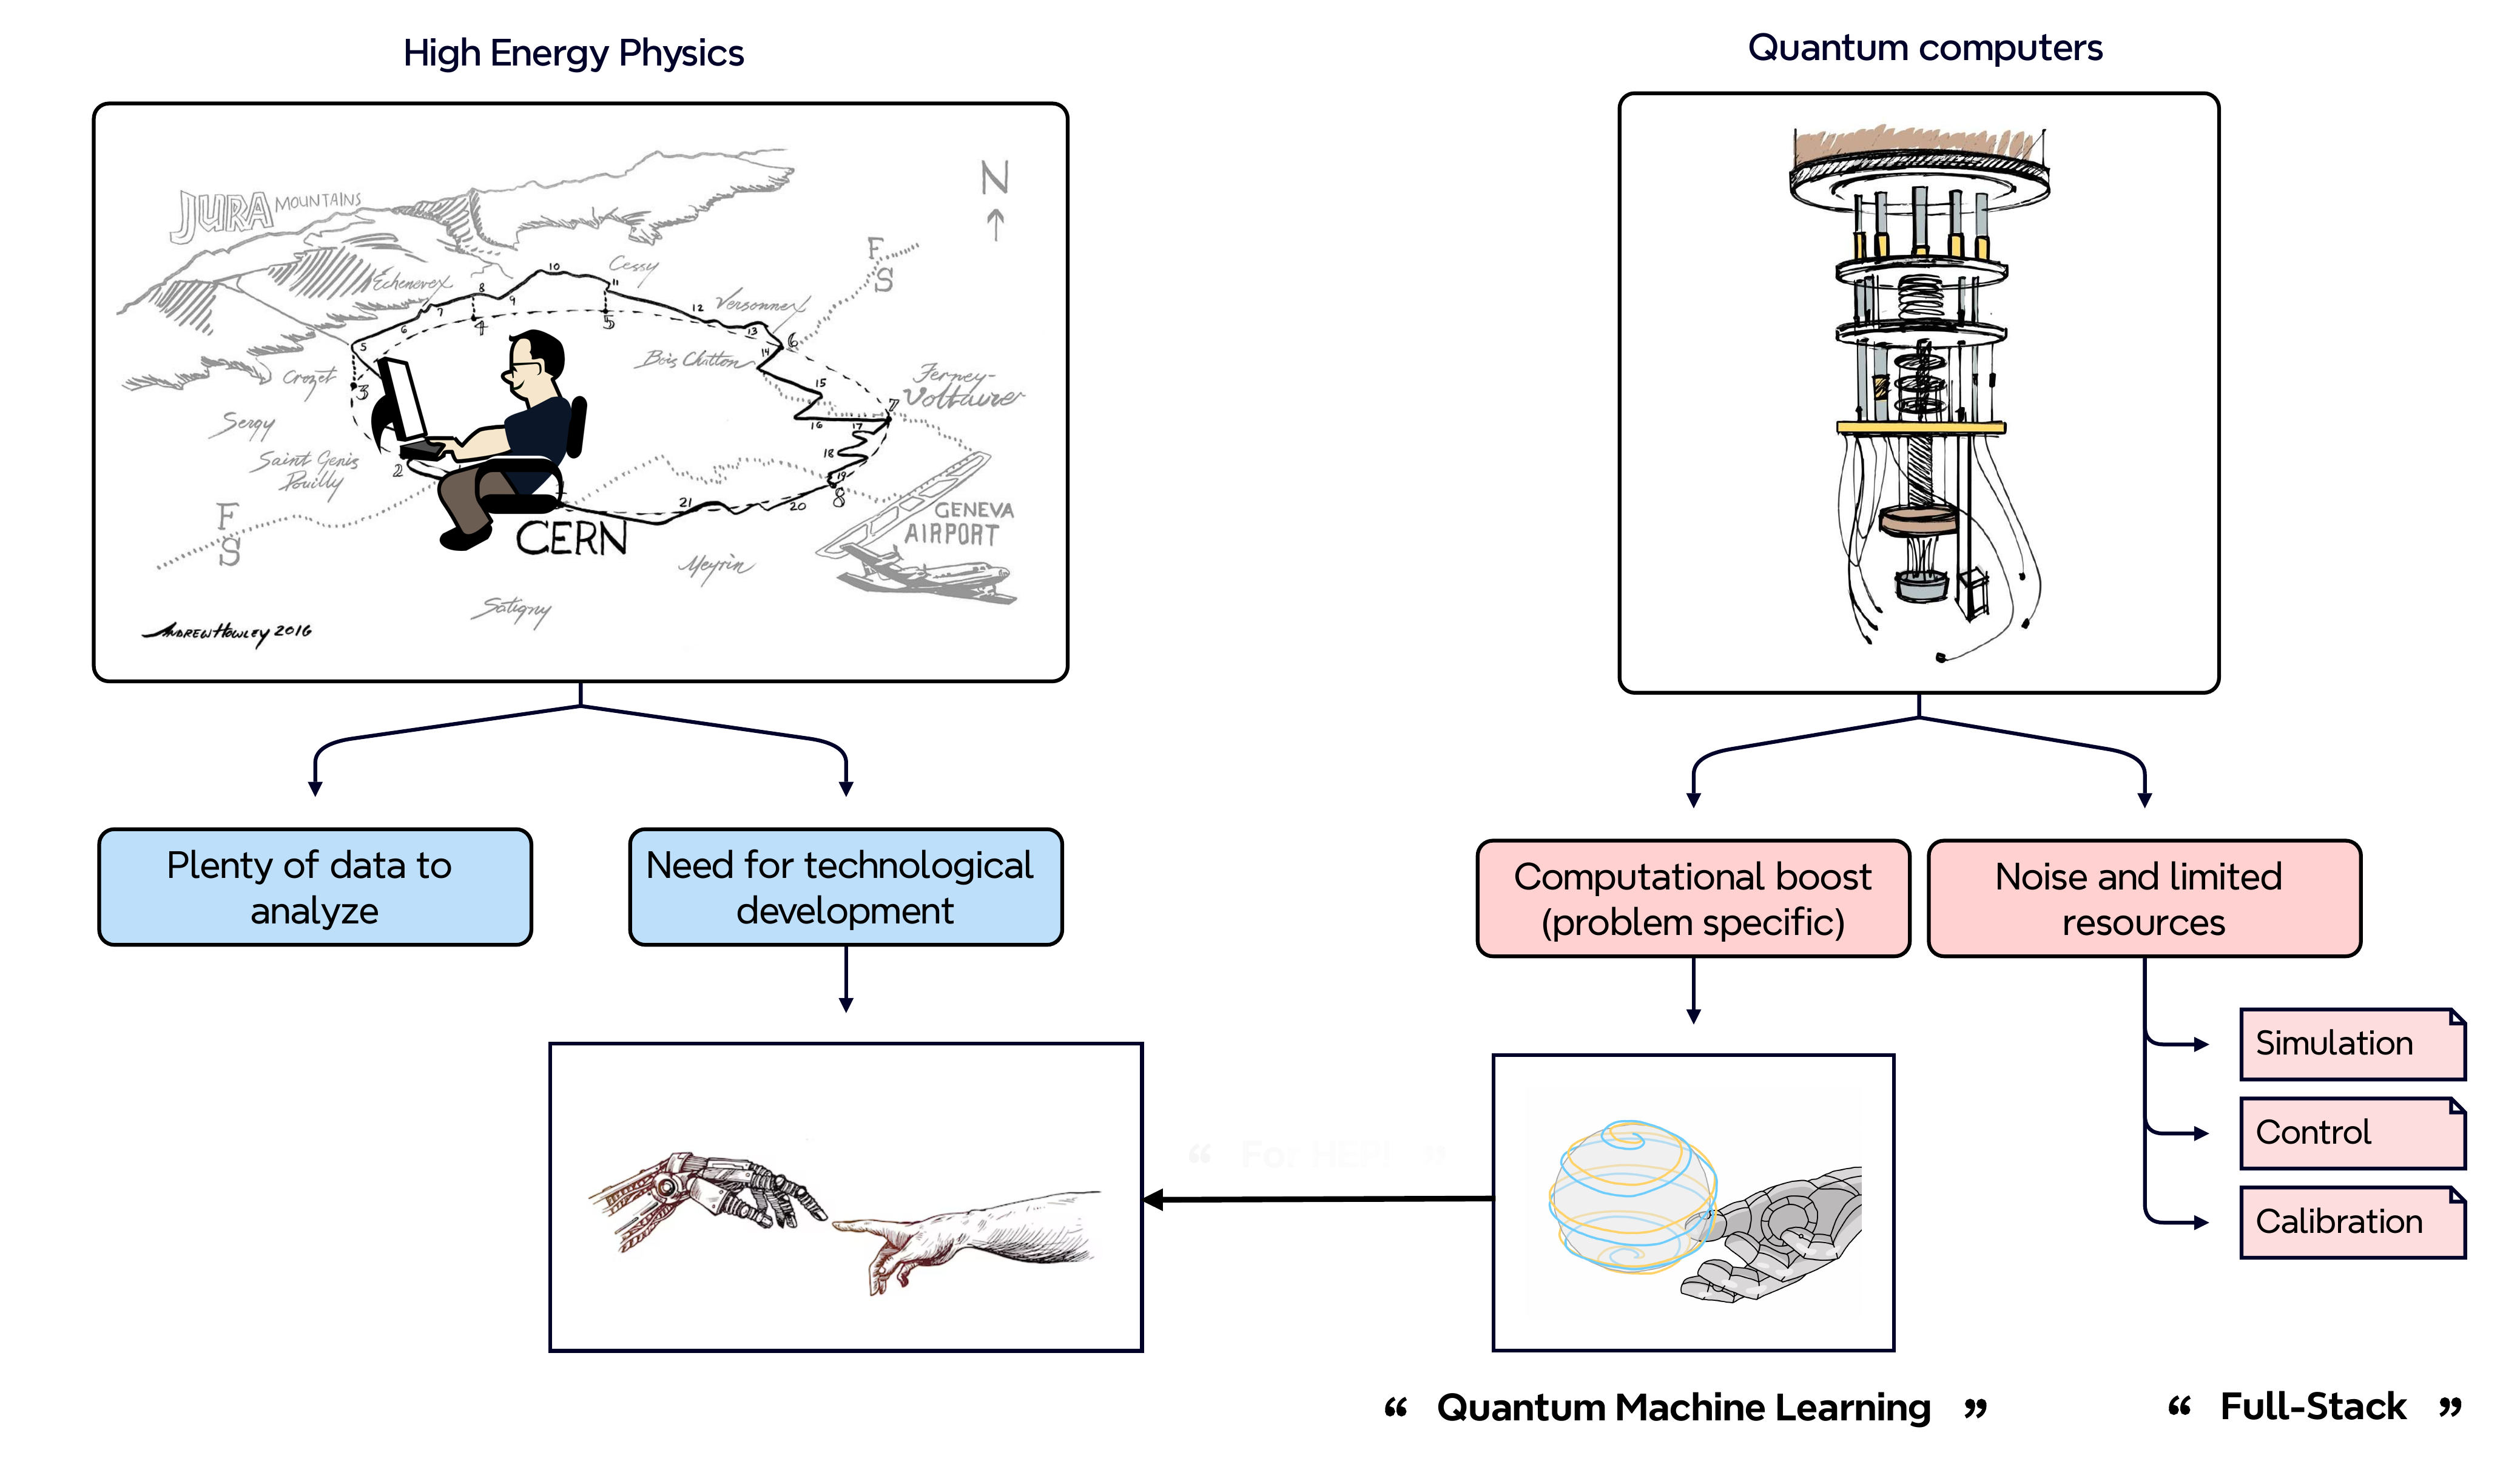
\includegraphics[width=1\textwidth]{figures/meinthecontext.png}
\end{figure}
\end{frame}

\section{Quantum Computing in a nutshell}



\begin{frame}{A quite general ``why?"}
\begin{figure}  
    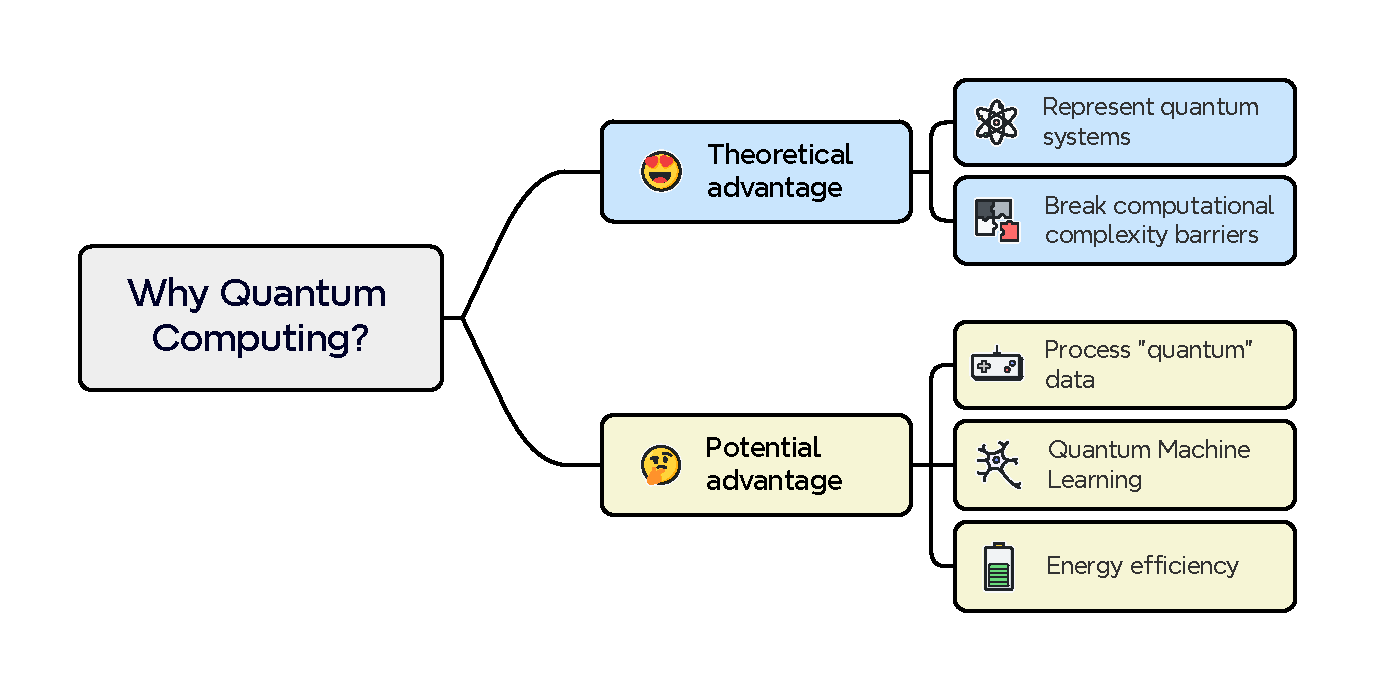
\includegraphics[width=1\textwidth]{figures/whyQC.pdf}
\end{figure}
\end{frame}

\begin{frame}{Gate based quantum computing}
        \begin{itemize}[noitemsep]
           \item<1,2,3,4>[1.] classical bits are replaced by \textbf{qubits}
           $ \ket{\psi} = \alpha\ket{0}+\beta\ket{1}$ (quantum states).
           \item<2,3,4>[2.] we can manipulate the qubit state applying \textbf{gates}: $\ket{\psi'}=\mathcal{U}(\bm{\theta})\ket{\psi}.$

           Typically we use 1-qubit and 2-qubits gates!
           \item<3,4>[3.] combine together gates to build \textbf{quantum circuits};
           \item<4>[4.] to access the information we need to measure the system.
        \end{itemize}
        \begin{figure}
            \only<1>{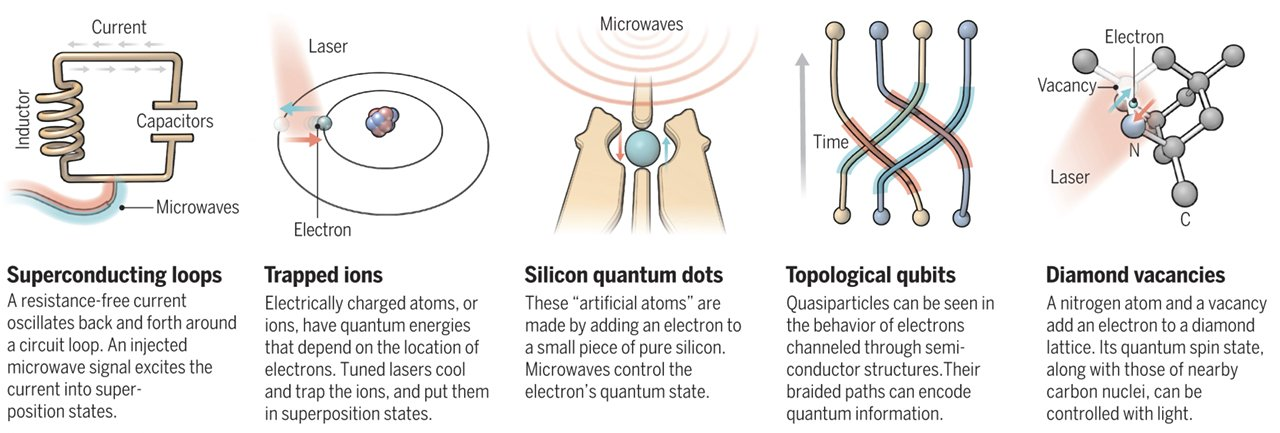
\includegraphics[width=0.7\linewidth, height=0.4\textheight]{figures/technologies.jpg}}%
            \only<2>{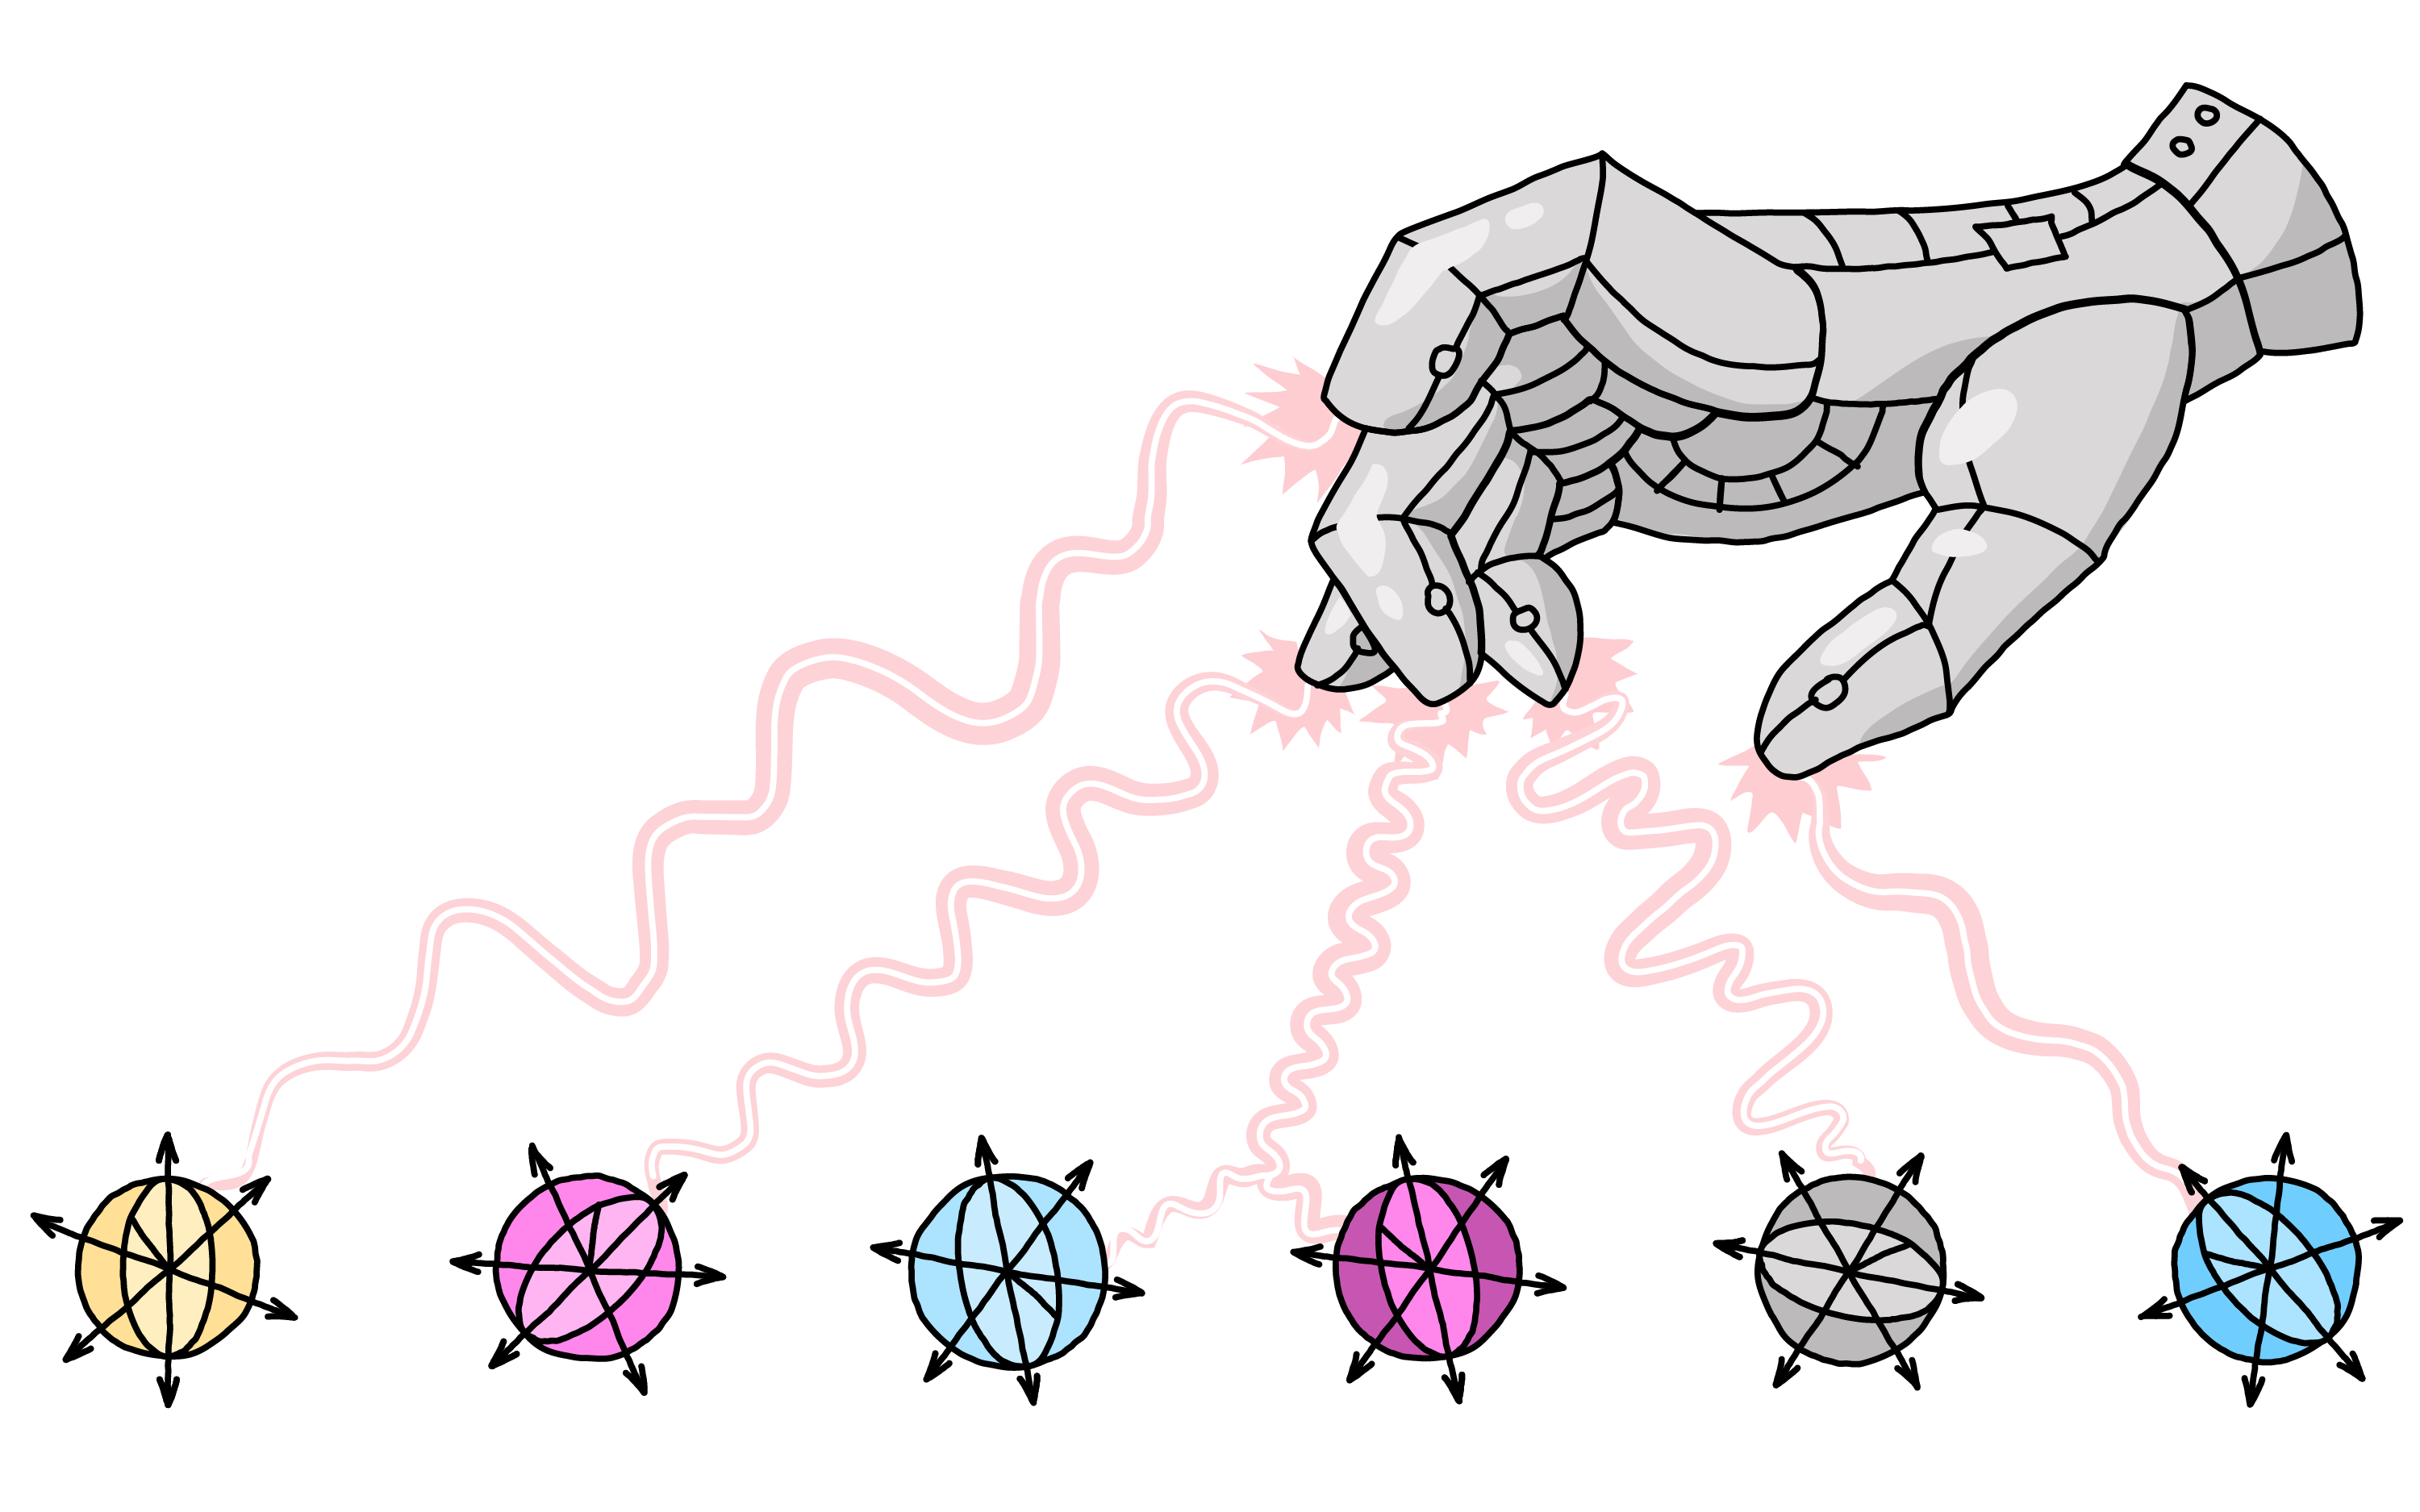
\includegraphics[width=0.4\linewidth, height=0.4\textheight]{figures/pulses.png}}%
            \only<3>{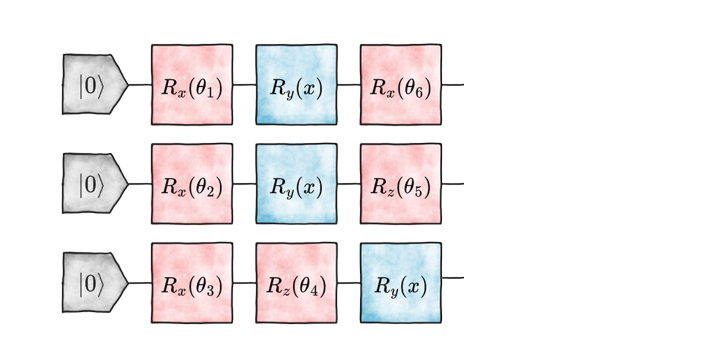
\includegraphics[width=0.5\linewidth, height=0.4\textheight]{figures/vqc_2.png}}
            \only<4>{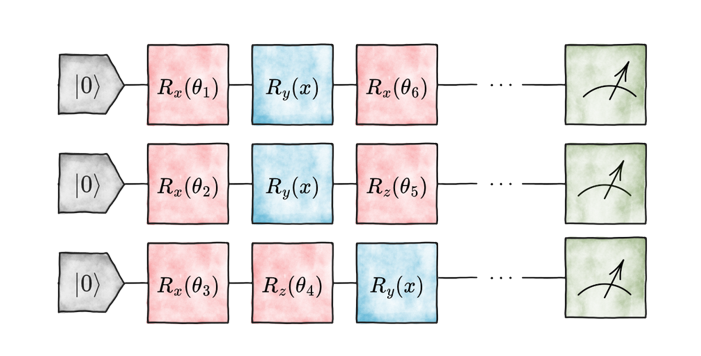
\includegraphics[width=0.5\linewidth, height=0.4\textheight]{figures/vqc.png}}
        \end{figure}        
\end{frame}


\begin{frame}{Example 1: preparing entangled states}

With quantum computing, we introduce new tools.
\begin{itemize}[noitemsep]
\item[\faRocket] prepare a quantum state in the computational zero $\ket{0}$;
\item[\faSliders] we can prepare superposition: 
$$H\ket{0} = \frac{1}{\sqrt{2}}(\ket{0} + \ket{1})  \quad \text{with} \quad H = \frac{1}{\sqrt{2}}
\begin{bmatrix} 1 & 1 \\ 1 & -1 \end{bmatrix},\,\, \ket{0}=\begin{bmatrix} 1 \\ 0 
\end{bmatrix},\,\,\ket{1}=\begin{bmatrix} 0 \\ 1 \end{bmatrix};$$
\item[\faShareAlt] let's apply a controlled-NOT (CNOT) gate on a second qubit prepared in $\ket{0}$:
$$ \text{CNOT} \biggl( \underbrace{\frac{1}{\sqrt{2}}(\ket{0} + \ket{1})}_{\text{control}}\otimes 
\ket{0} \biggr) = \frac{1}{\sqrt{2}}(\ket{\textcolor{bleudefrance}{0}0} + 
\text{NOT}_{\rm targ}\ket{\textcolor{brightmaroon}{1}0}) = \frac{1}{\sqrt{2}}(\ket{00} + \ket{11}). $$
\end{itemize}
\pause
\begin{multicols}{2}
\texttt{\\}
\begin{figure}
   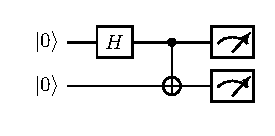
\includegraphics[width=.8\linewidth]{figures/baby3.pdf} %
   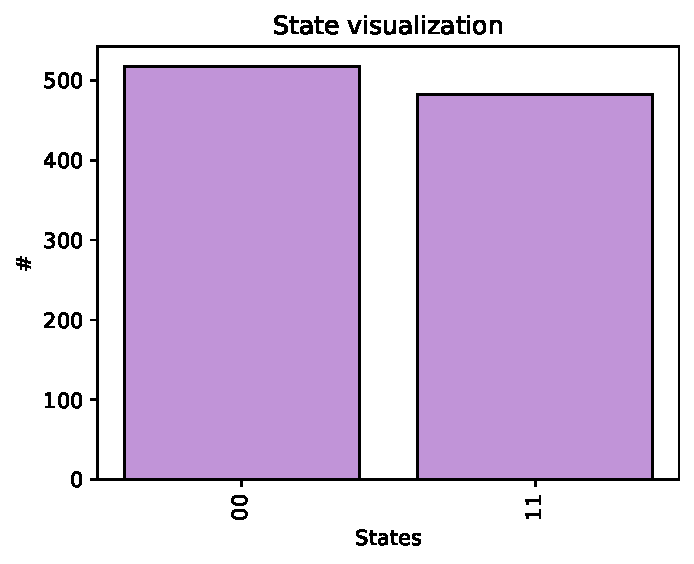
\includegraphics[width=.6\linewidth]{figures/bell.pdf} %
\end{figure}   
\end{multicols} 
\end{frame}

\begin{frame}{Parametric gates prepare variational quantum states}
\begin{itemize}[noitemsep]
\item[\faLightbulbO] Among the gates, parametric ones can be useful!
\item[\faMapPin] Let's consider a single qubit system:
\begin{equation*}
   \ket{\psi} = \alpha\ket{0}+\beta\ket{1} \qquad \text{with}
   \qquad \alpha = \cos{\frac{\theta}{2}}, \quad \beta = e^{i\phi}\sin{\frac{\theta}{2}}.
\end{equation*}
\end{itemize}
\begin{center}
\begin{multicols}{2}
\def\rotationSphere{-110}
\def\radiusSphere{1.8cm}
\def\psiLat{45}
\def\psiLon{45}
\begin{blochsphere}[radius=\radiusSphere,opacity=0,rotation=\rotationSphere]
  % \drawBallGrid[style={opacity=.3}]{30}{45}
  % Draw the sphere...
  \drawLongitudeCircle[]{\rotationSphere}

  \drawLatitudeCircle[style={dashed}]{0}
  % Define the different points on the bloch sphere
  \labelLatLon{ket0}{90}{0};
  \labelLatLon{ket1}{-90}{0};
  \labelLatLon{ketminus}{0}{180};
  \labelLatLon{ketplus}{00}{0};
  \labelLatLon{ketpluspi2}{0}{-90};  % Longitude seems to be defined in the "wrong" direction, hence the minus
  \labelLatLon{ketplus3pi2}{0}{-270};
  \labelLatLon{psi}{\psiLat}{-\psiLon};
  % Draw and label the axis
  \draw[-latex] (0,0) -- (ket0) node[above,inner sep=.5mm] at (ket0) {\footnotesize $z$};
  \draw[-latex] (0,0) -- (ketplus) node[below,inner sep=.5mm] at (ketplus) {\footnotesize$x$};
  \draw[-latex] (0,0) -- (ketpluspi2) node[below,inner sep=.5mm] at (ketpluspi2) {\footnotesize $y$};
  % Draw |psi>
  \draw[-latex] (0,0) -- (psi) node[above]{\footnotesize $\ket{\psi}$};

  % Draw the angles
  \coordinate (origin) at (0,0);
  {
    % Will draw the angle/projection one the equatorial plane
    \setDrawingPlane{0}{0}
    % Draw the projection: cos is used to compute the length of the projection
    \draw[current plane,dashed] (0,0) -- (-90+\psiLon:{cos(\psiLat)*\radiusSphere}) coordinate (psiProjectedEquat) -- (psi);
    % Draw the angle
    \pic[current plane, draw,fill=purple!50,fill opacity=.5, text opacity=1,"\footnotesize $\phi$", angle eccentricity=2.2]{angle=ketplus--origin--psiProjectedEquat};
  }
  { \setLongitudinalDrawingPlane{\psiLon}
    % Draw the angle
    \pic[current plane, draw,fill=purple!50,fill opacity=.5, text opacity=1,"\footnotesize $\xi$", angle eccentricity=1.5]{angle=psi--origin--ket0};
  }
\end{blochsphere}


\def\rotationSphere{-110}
\def\radiusSphere{1.8cm}
\def\psiLat{45}
\def\psiLon{45}
\def\psiLatPrime{15} % Adjusted latitude for \psi' to be at the top
\def\psiLonPrime{-15} % Adjusted longitude for \psi' to be on the left-top

\begin{blochsphere}[radius=\radiusSphere, opacity=0, rotation=\rotationSphere]
  \drawLongitudeCircle[]{\rotationSphere}
  \drawLatitudeCircle[style={dashed}]{0}

  \labelLatLon{ket0}{90}{0};
  \labelLatLon{ket1}{-90}{0};
  \labelLatLon{ketminus}{0}{180};
  \labelLatLon{ketplus}{00}{0};
  \labelLatLon{ketpluspi2}{0}{-90};
  \labelLatLon{ketplus3pi2}{0}{-270};
  \labelLatLon{psi}{\psiLat}{-\psiLon};
  \labelLatLon{psiPrime}{\psiLatPrime}{-\psiLonPrime};

  \draw[-latex] (0,0) -- (ket0) node[above,inner sep=.5mm] at (ket0) {\footnotesize $z$};
  \draw[-latex] (0,0) -- (ketplus) node[below,inner sep=.5mm] at (ketplus) {\footnotesize$x$};
  \draw[-latex] (0,0) -- (ketpluspi2) node[below,inner sep=.5mm] at (ketpluspi2) {\footnotesize $y$};
  \draw[-latex, purple] (0,0) -- (psi) node[right, black]{\footnotesize $\ket{\psi}$};
  \draw[-latex, purple] (0,0) -- (psiPrime) node[left, black]{\footnotesize $\ket{\psi'}$};


% Draw modified trajectory with two curves before reaching psi'
\draw[purple, thick, ->] (psi) to[out=110, in=20] ++(-1,0.5) to[out=200, in=60] ++(0.3,-0.3) to[out=240, in=100] ++(-0.5,-0.3) to[out=280, in=100] (psiPrime);
\node[purple] at (-1,1) {$\mathcal{U}(\theta)$};
\end{blochsphere}
\end{multicols}
\end{center}
\vspace{-0.3cm}
We can use as parametric gates the rotation around the axis of the block sphere:
$$ R_k(\theta) = \text{exp}\bigl[-i \theta \sigma_k\bigr], \qquad \text{with} \qquad
\sigma_k \in \{I, \sigma_x, \sigma_y, \sigma_z\}. $$
\end{frame}

\begin{frame}{Parametric quantum circuits}
Parametric gates can be used to build parametric quantum circuits.
\begin{figure}
   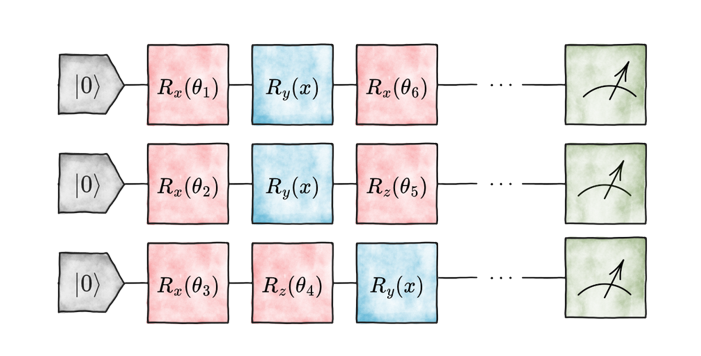
\includegraphics[width=0.7\linewidth]{figures/vqc.png}
\end{figure}  
\end{frame}


\section{\texttt{Qibo 0.2.8}}

\begin{frame}{What is needed for doing quantum computing?}
\begin{figure}
   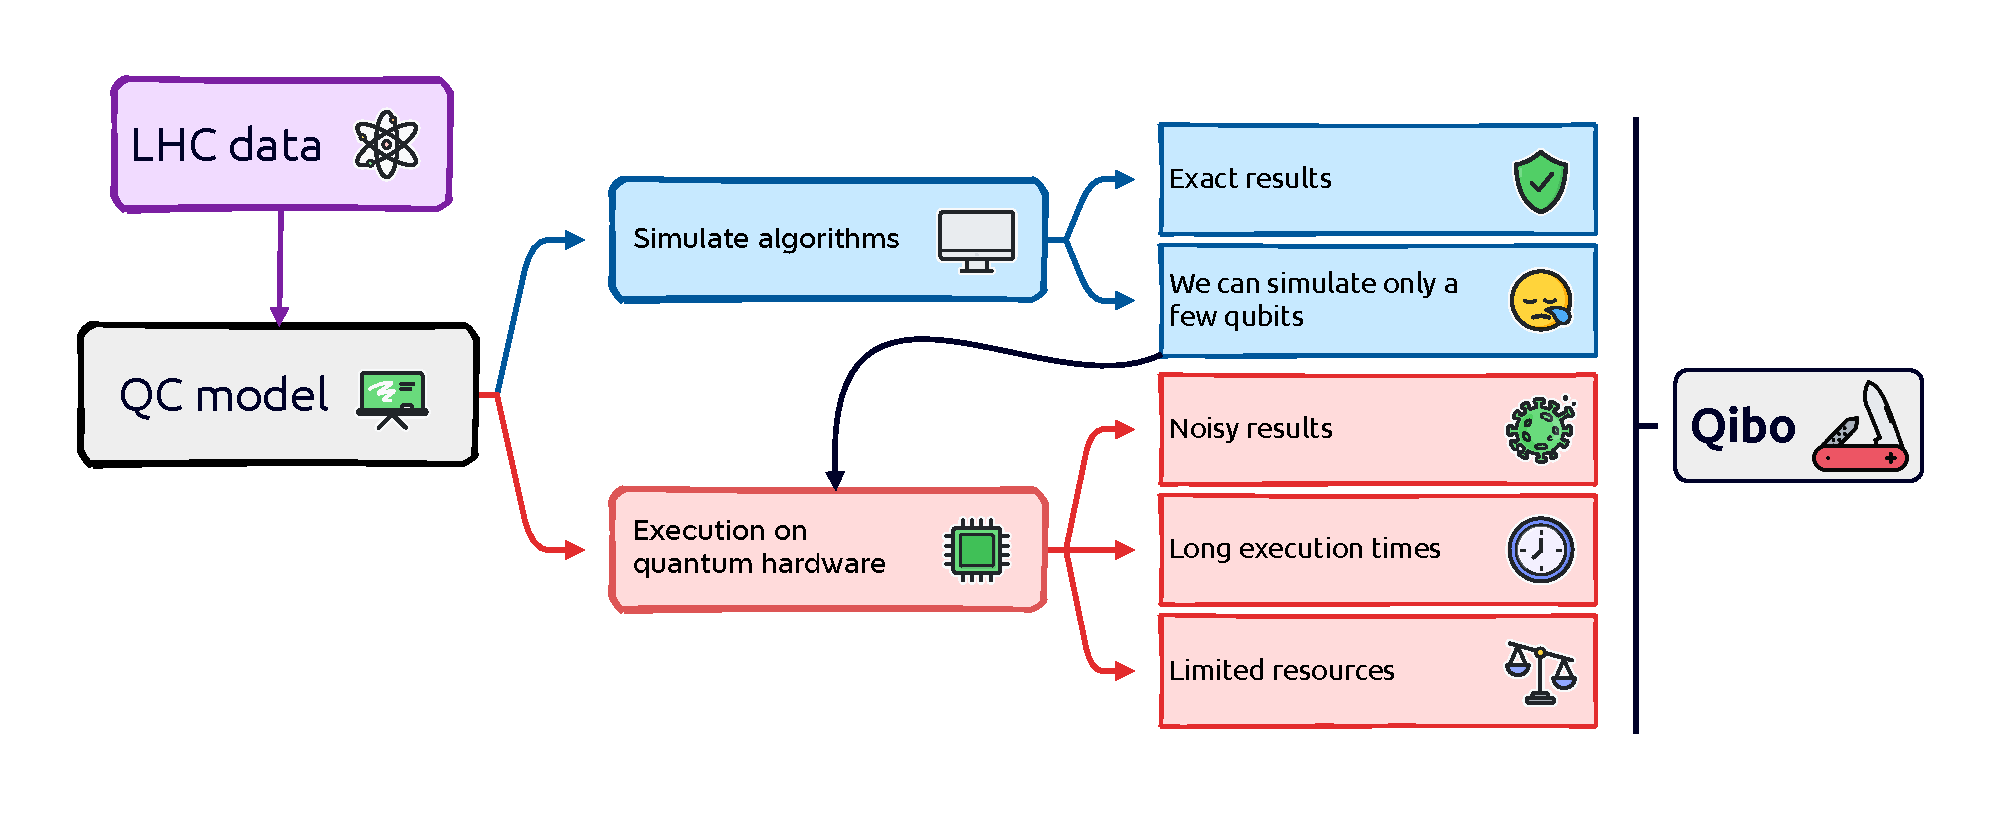
\includegraphics[width=1\linewidth]{figures/qc_onchip.pdf}
\end{figure}  
\end{frame}

\begin{frame}{The Qibo ecosystem\hfill \faBook\,\, \href{https://arxiv.org/abs/2009.01845}{arXiv:2009.01845}}

   \textbf{Qibo} is an \textbf{open-source} hybrid quantum operating system for self-hosted quantum computers.
   \begin{columns}
     \column{6cm}
     \begin{figure}
       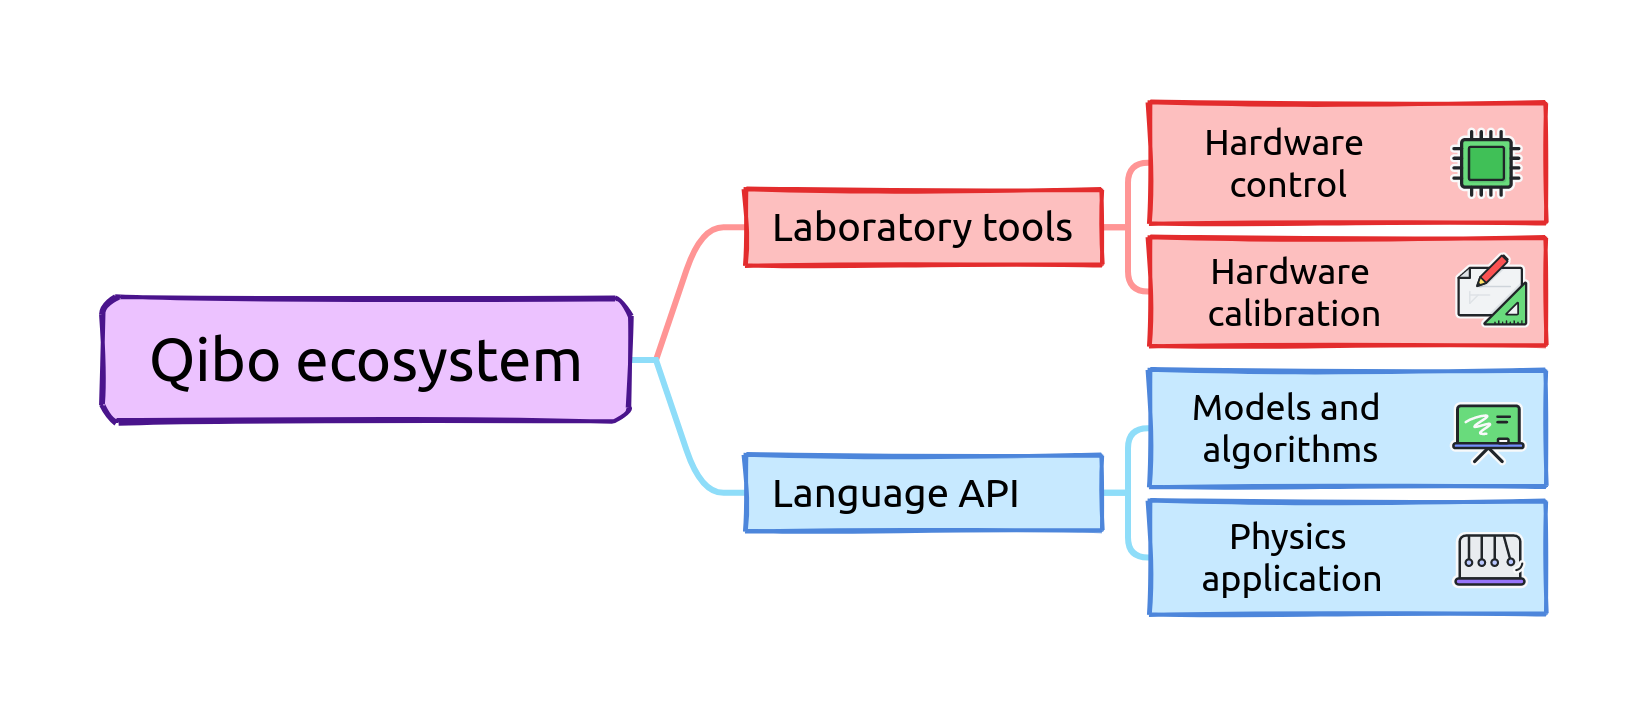
\includegraphics[width=1\textwidth]{figures/overview.png}
     \end{figure}
     \vspace{-0.5cm}
   \begin{itemize}
     \item[1.] Fully open-source and community driven.
     \item[2.] Modular layout design with possibility of adding:
     \begin{itemize}[noitemsep]
       \item[-] new backends for simulation,
       \item[-] new platforms for hardware control,
       \item[-] new drivers for control electronics.
     \end{itemize}
     \item[3.] Supported by documentation and tests/CI on quantum hardware.
   \end{itemize}

     \column{4cm}
     \begin{figure}
       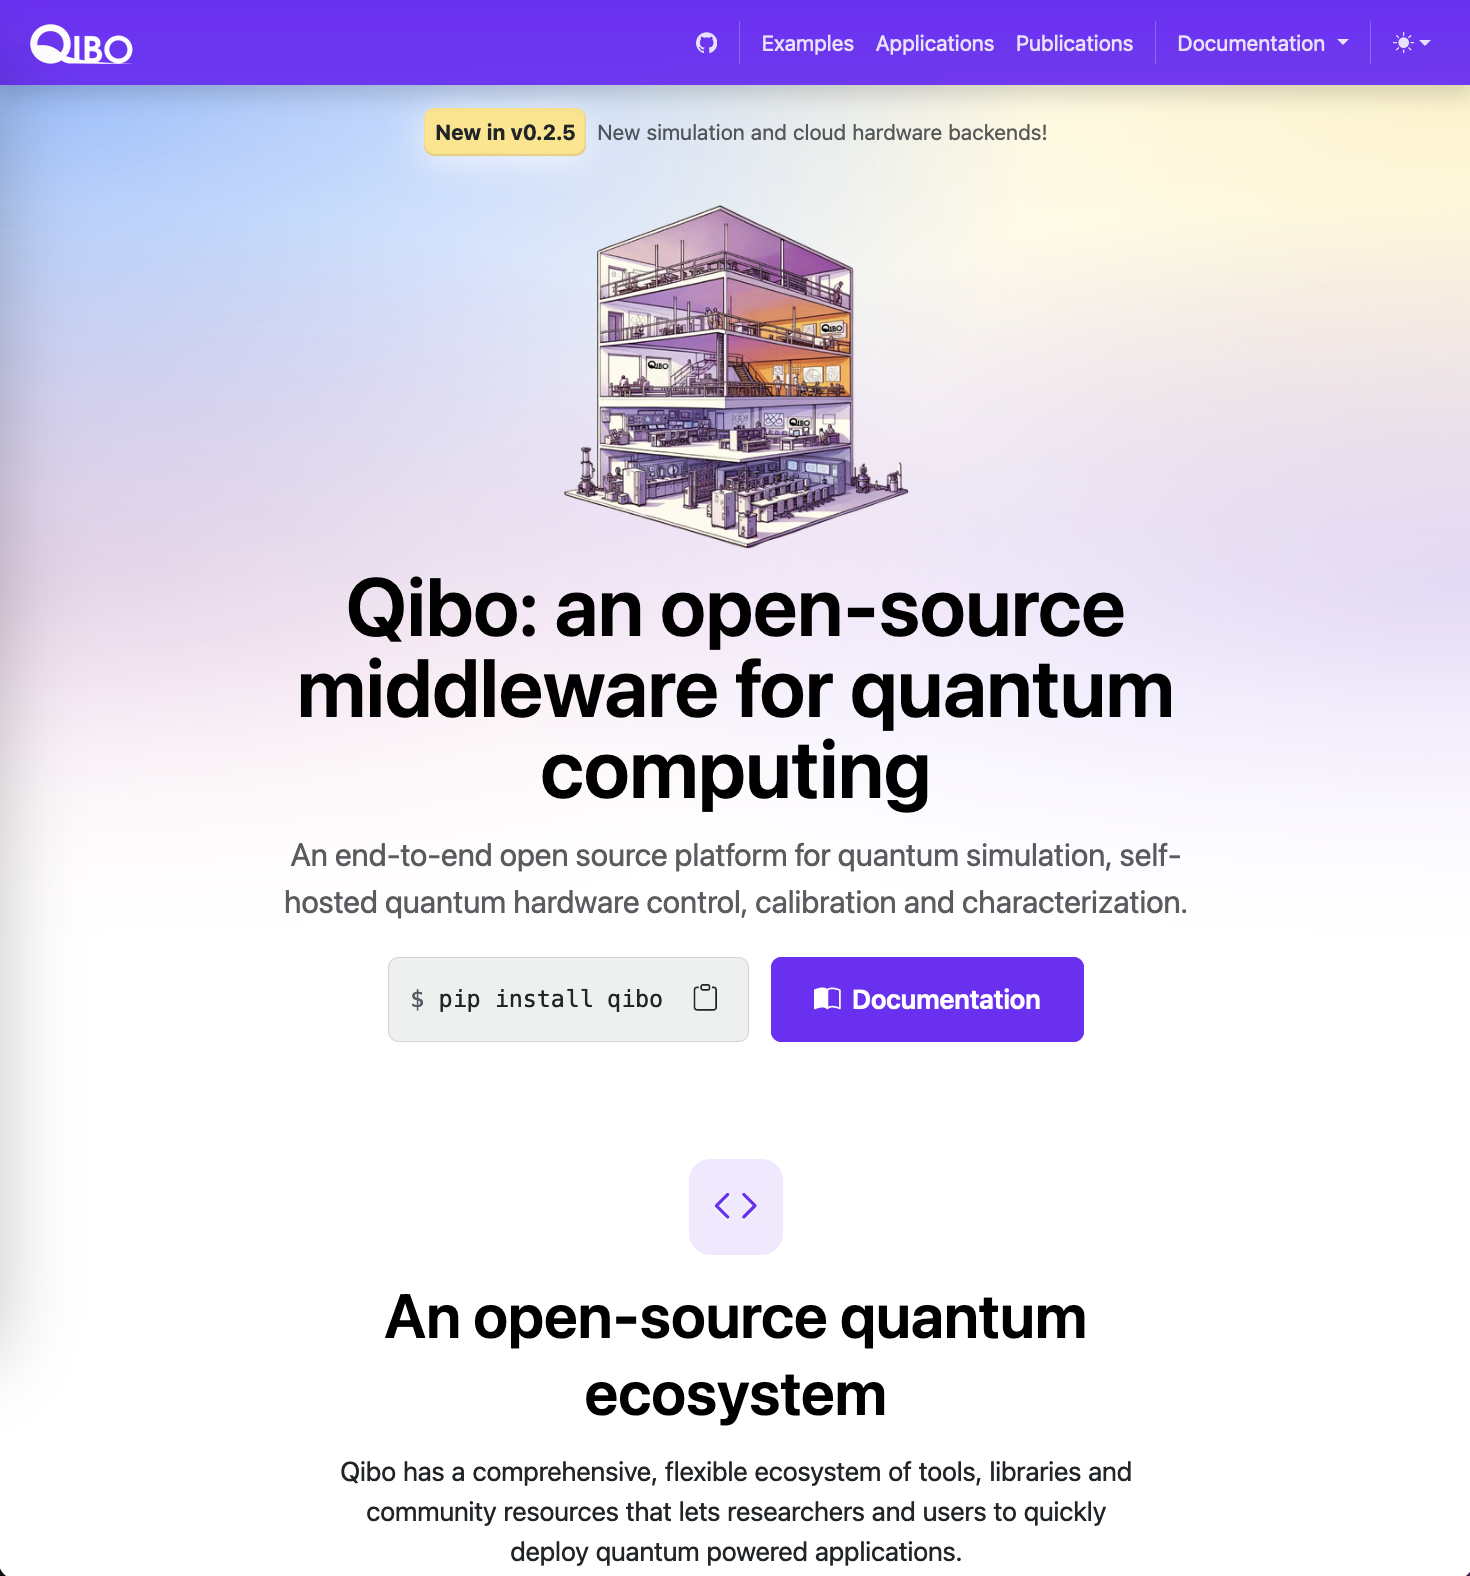
\includegraphics[width=\textwidth]{figures/docs.png}
       {\color{blue}\url{https://qibo.science}}
     \end{figure}
   \end{columns}
\end{frame}

\begin{frame}{The Qibo timeline}
\begin{figure}
   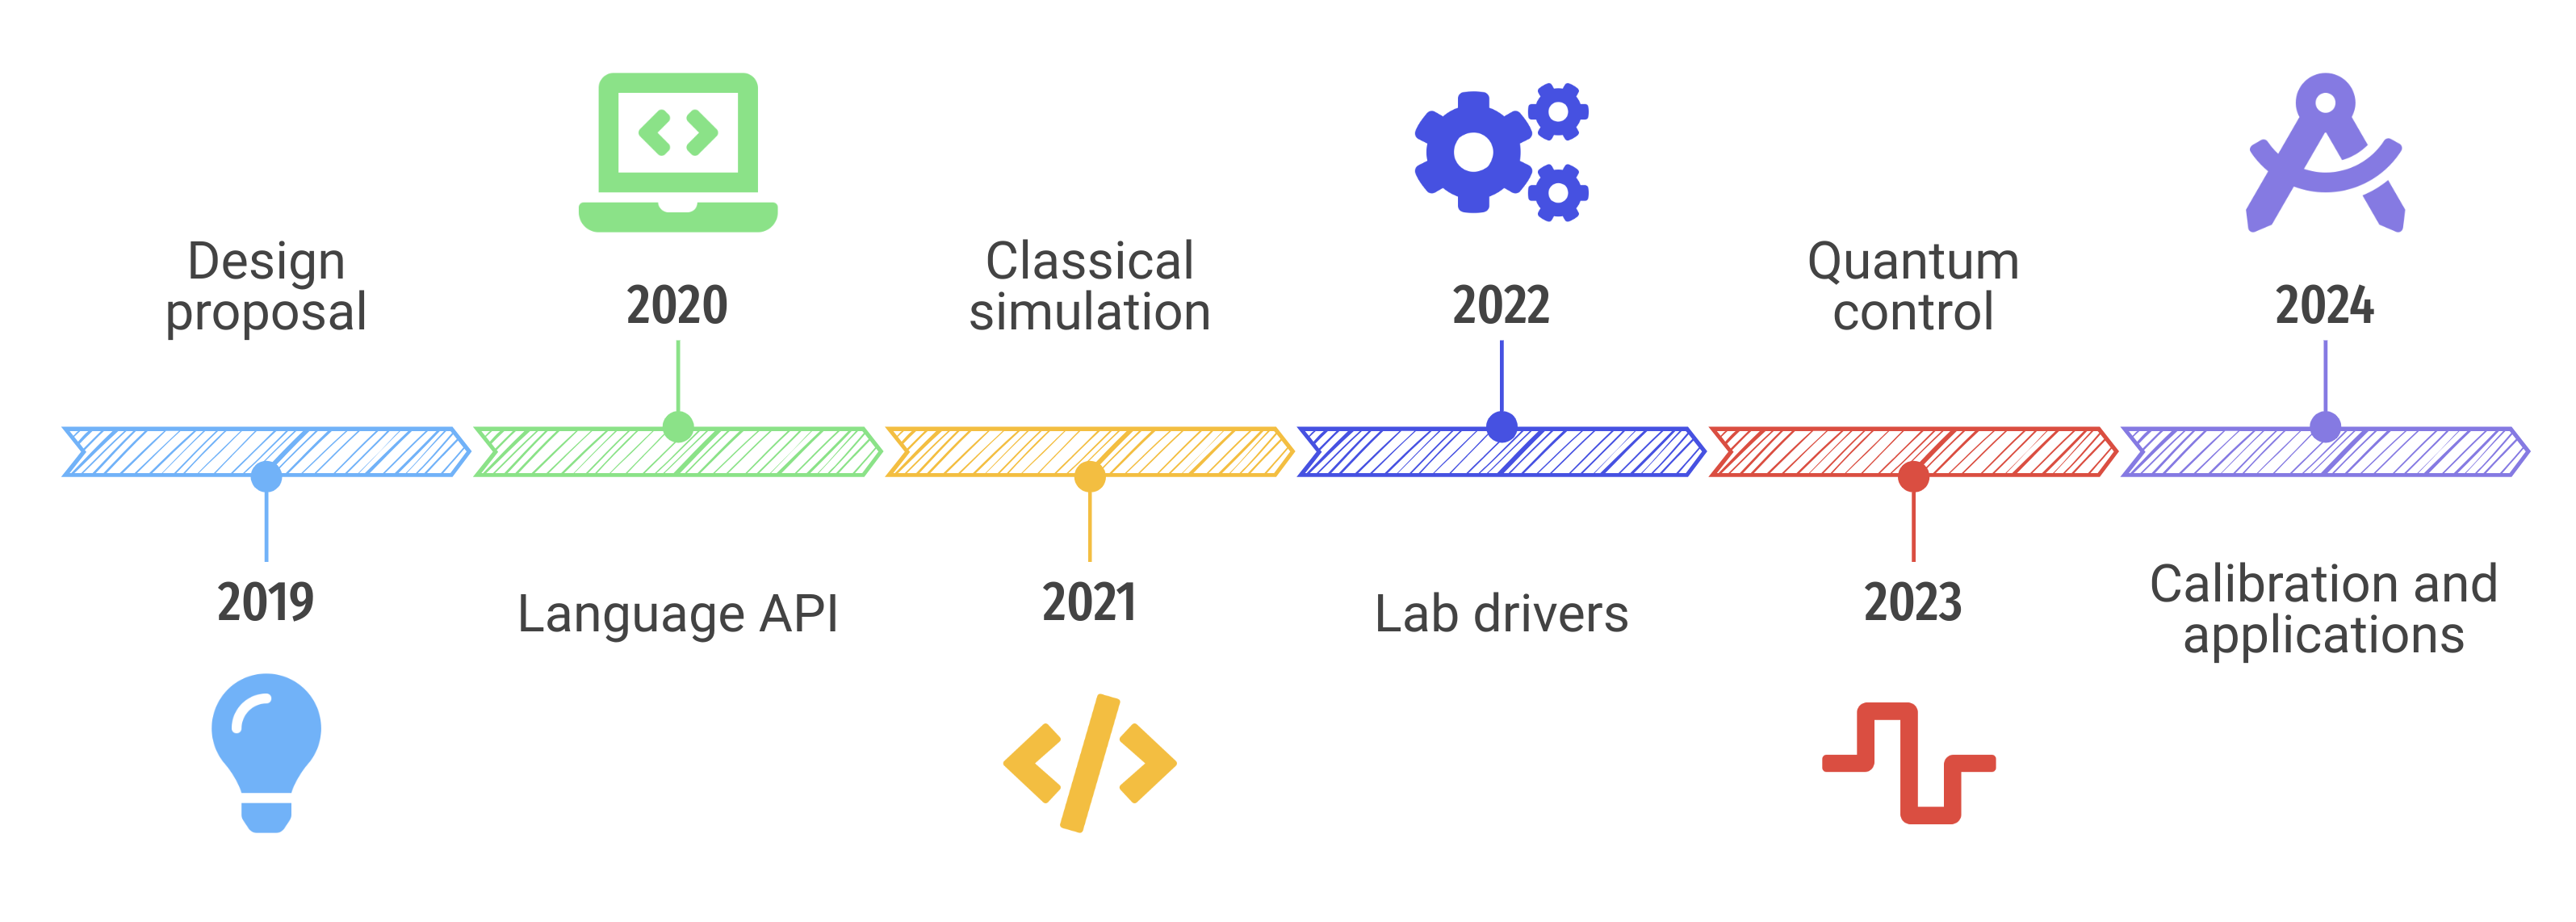
\includegraphics[width=1\linewidth]{figures/timeline.png}
\end{figure}  
\end{frame}

\begin{frame}{An open source and full-stack framework for QC \hfill \href{https://arxiv.org/abs/2308.06313}{\faBook\,\,	arXiv:2308.06313}}
\begin{figure}
   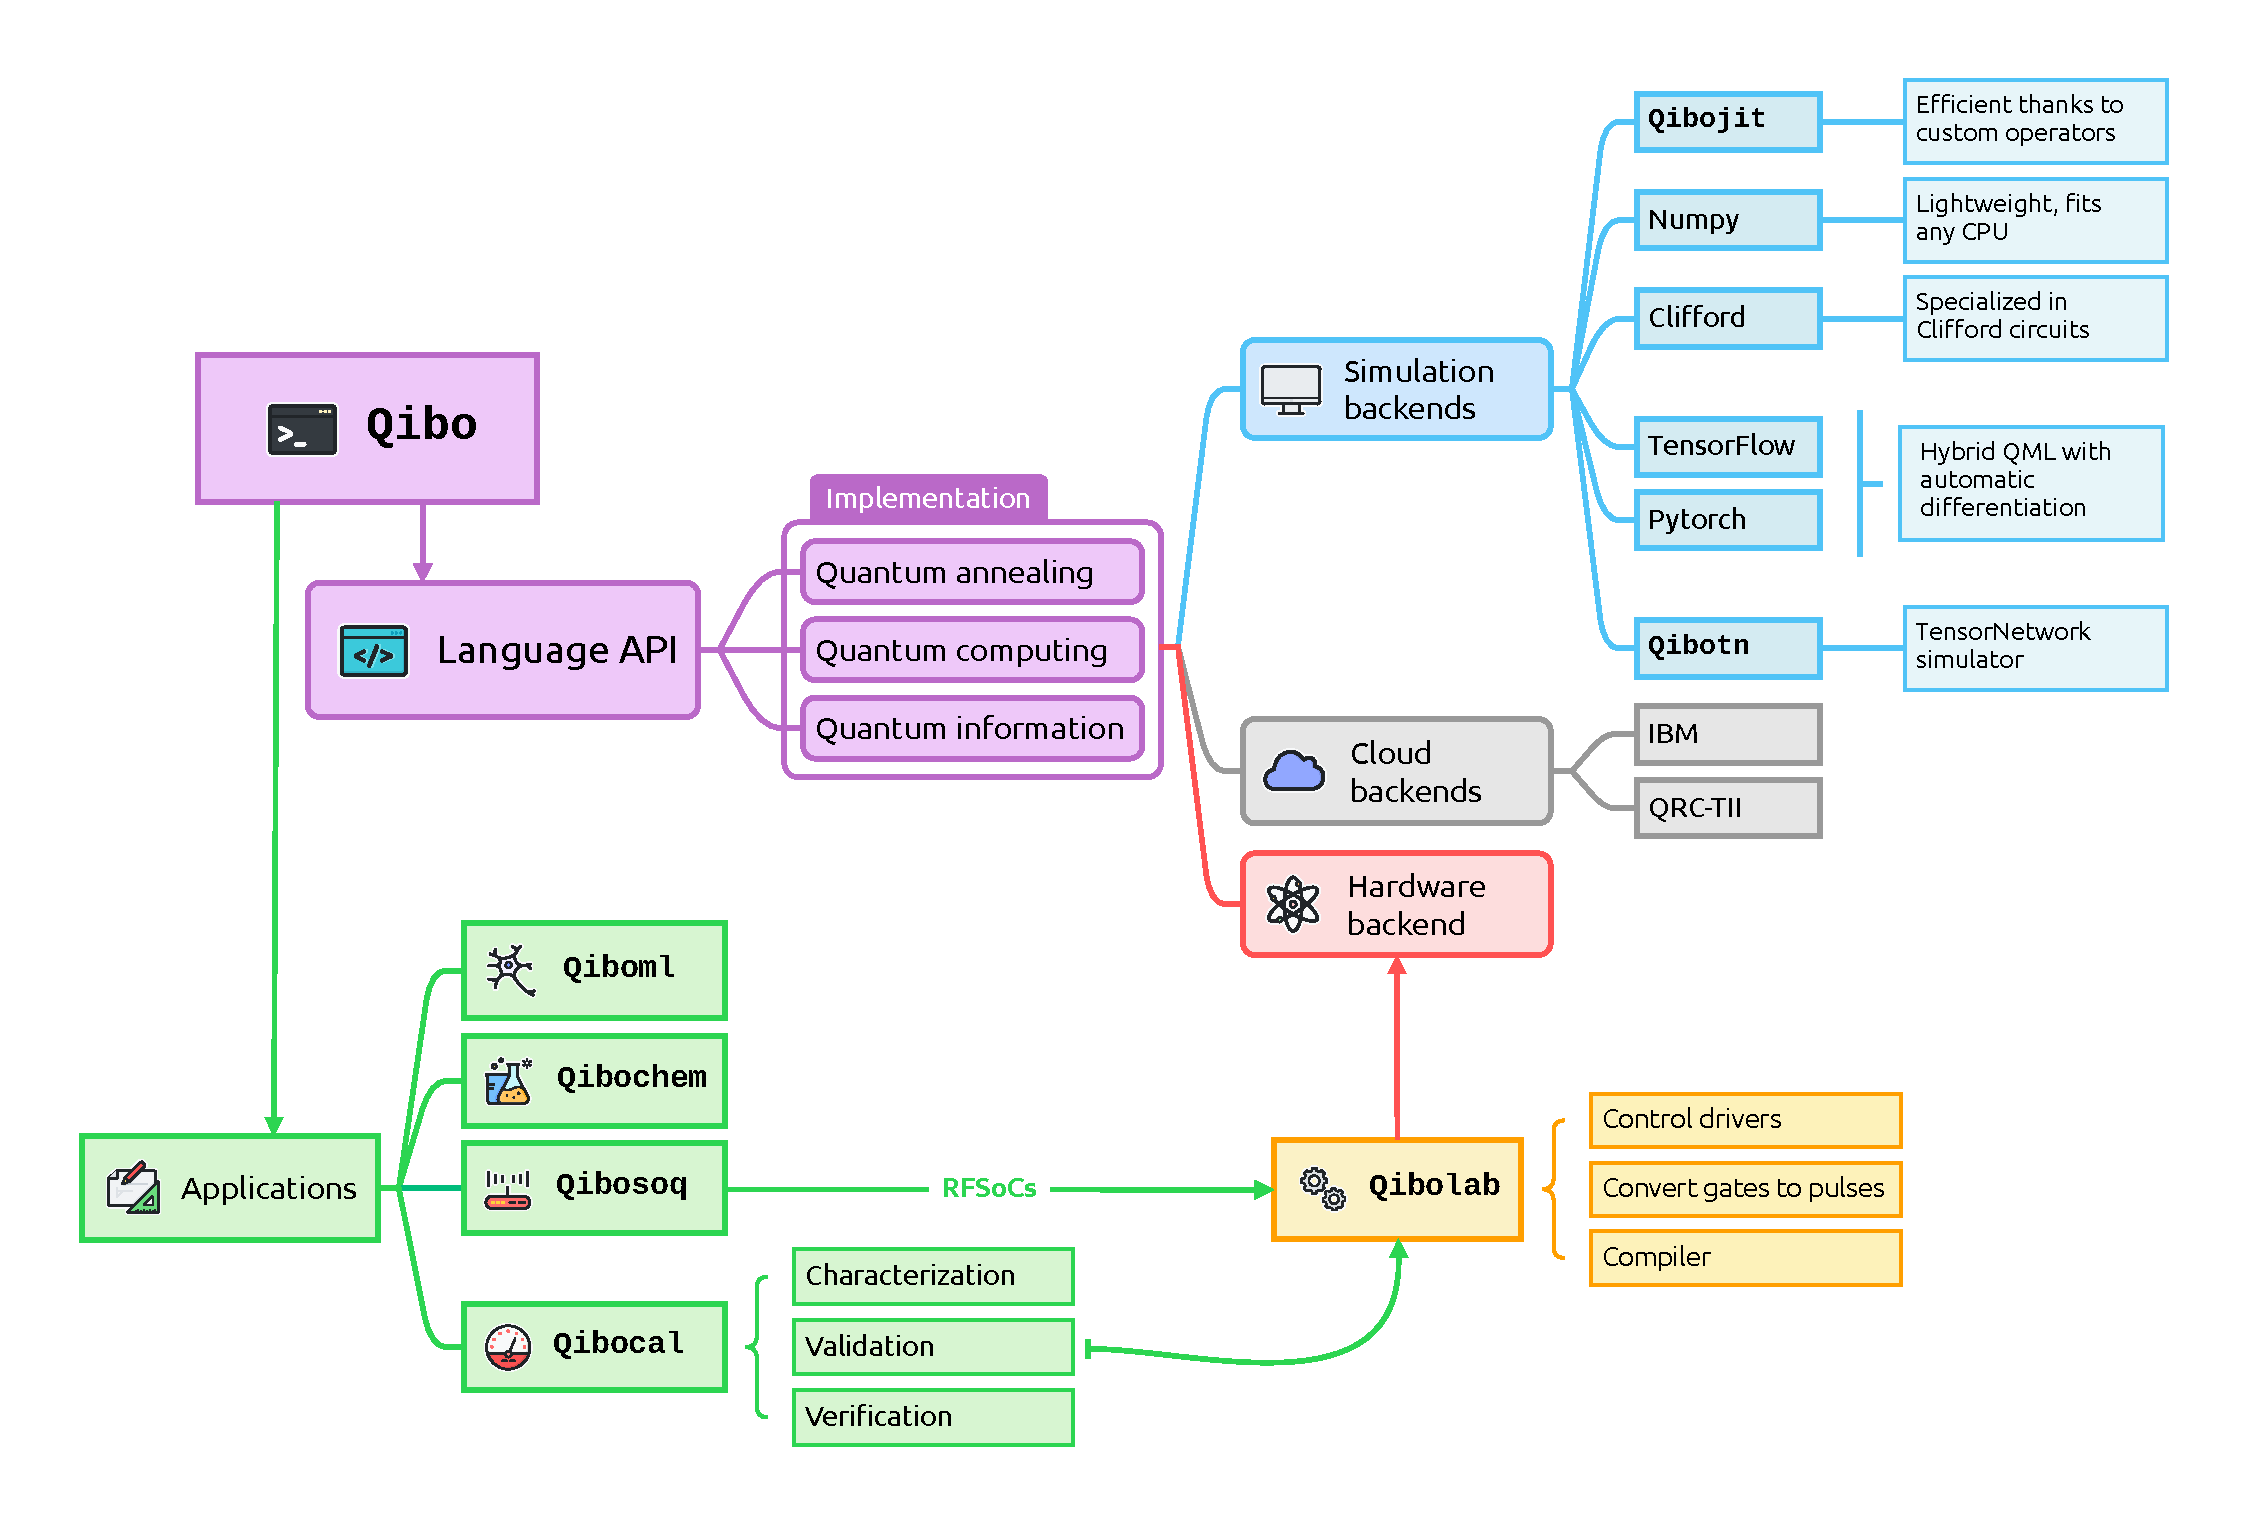
\includegraphics[width=0.8\linewidth]{figures/qibo_ecosystem.pdf}
\end{figure}  
\vspace{-0.8cm}
\hfill \href{https://github.com/qiboteam}{\faGithub ~ https://github.com/qiboteam}
\end{frame}

\begin{frame}{A focus on classical simulation performances \hfill \href{https://arxiv.org/abs/2203.08826}{\faBook\,\,arXiv:2203.08826}}
State vector simulation solves:
   \begin{equation*}
     \psi' (\sigma_1,\ldots,\sigma_n) = \sum_{\boldsymbol \tau'} G({\boldsymbol \tau},{\boldsymbol \tau}') \psi(\sigma_1,\ldots,{\boldsymbol \tau}',\ldots,\sigma_n)
   \end{equation*}
   The number of operations scales {\color{magenta} exponentially} with the number of qubits.

   \textbf{Qibo} uses just-in-time technology and hardware acceleration:
   \vspace{-0.35cm}
   \begin{figure}
     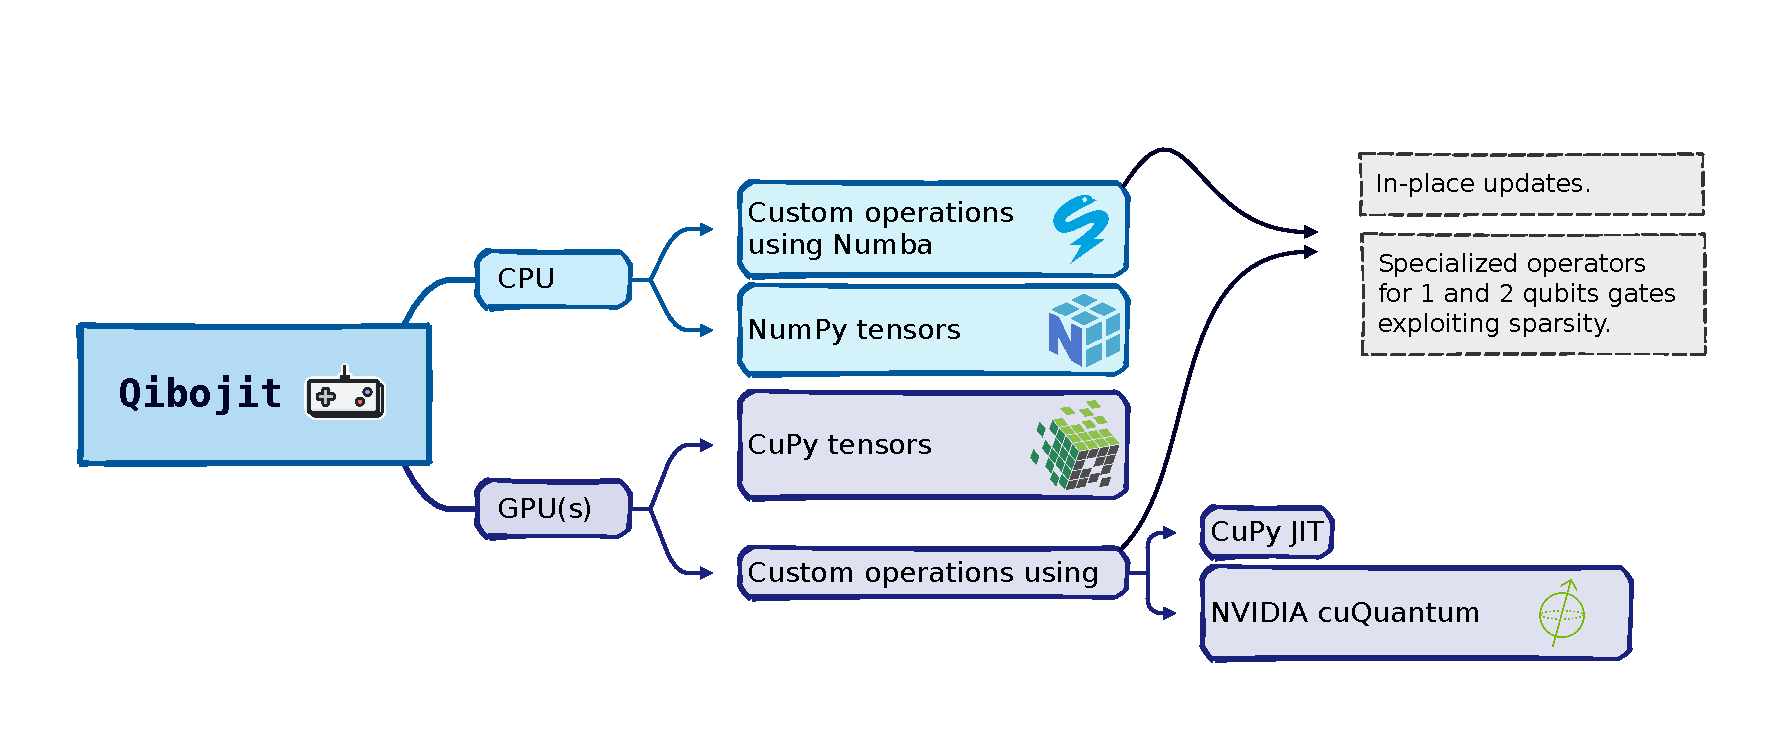
\includegraphics[height=4.5cm]{figures/qibojit.pdf}
   \end{figure}

\end{frame}

\begin{frame}{A focus on classical simulation performances \hfill \href{https://arxiv.org/abs/2203.08826}{\faBook\,\,arXiv:2203.08826}}

Through its modularity, \texttt{Qibo} allows execution of the same high level language onto 
different classical hardware accellerators.
\begin{multicols}{2}
   \begin{figure}
     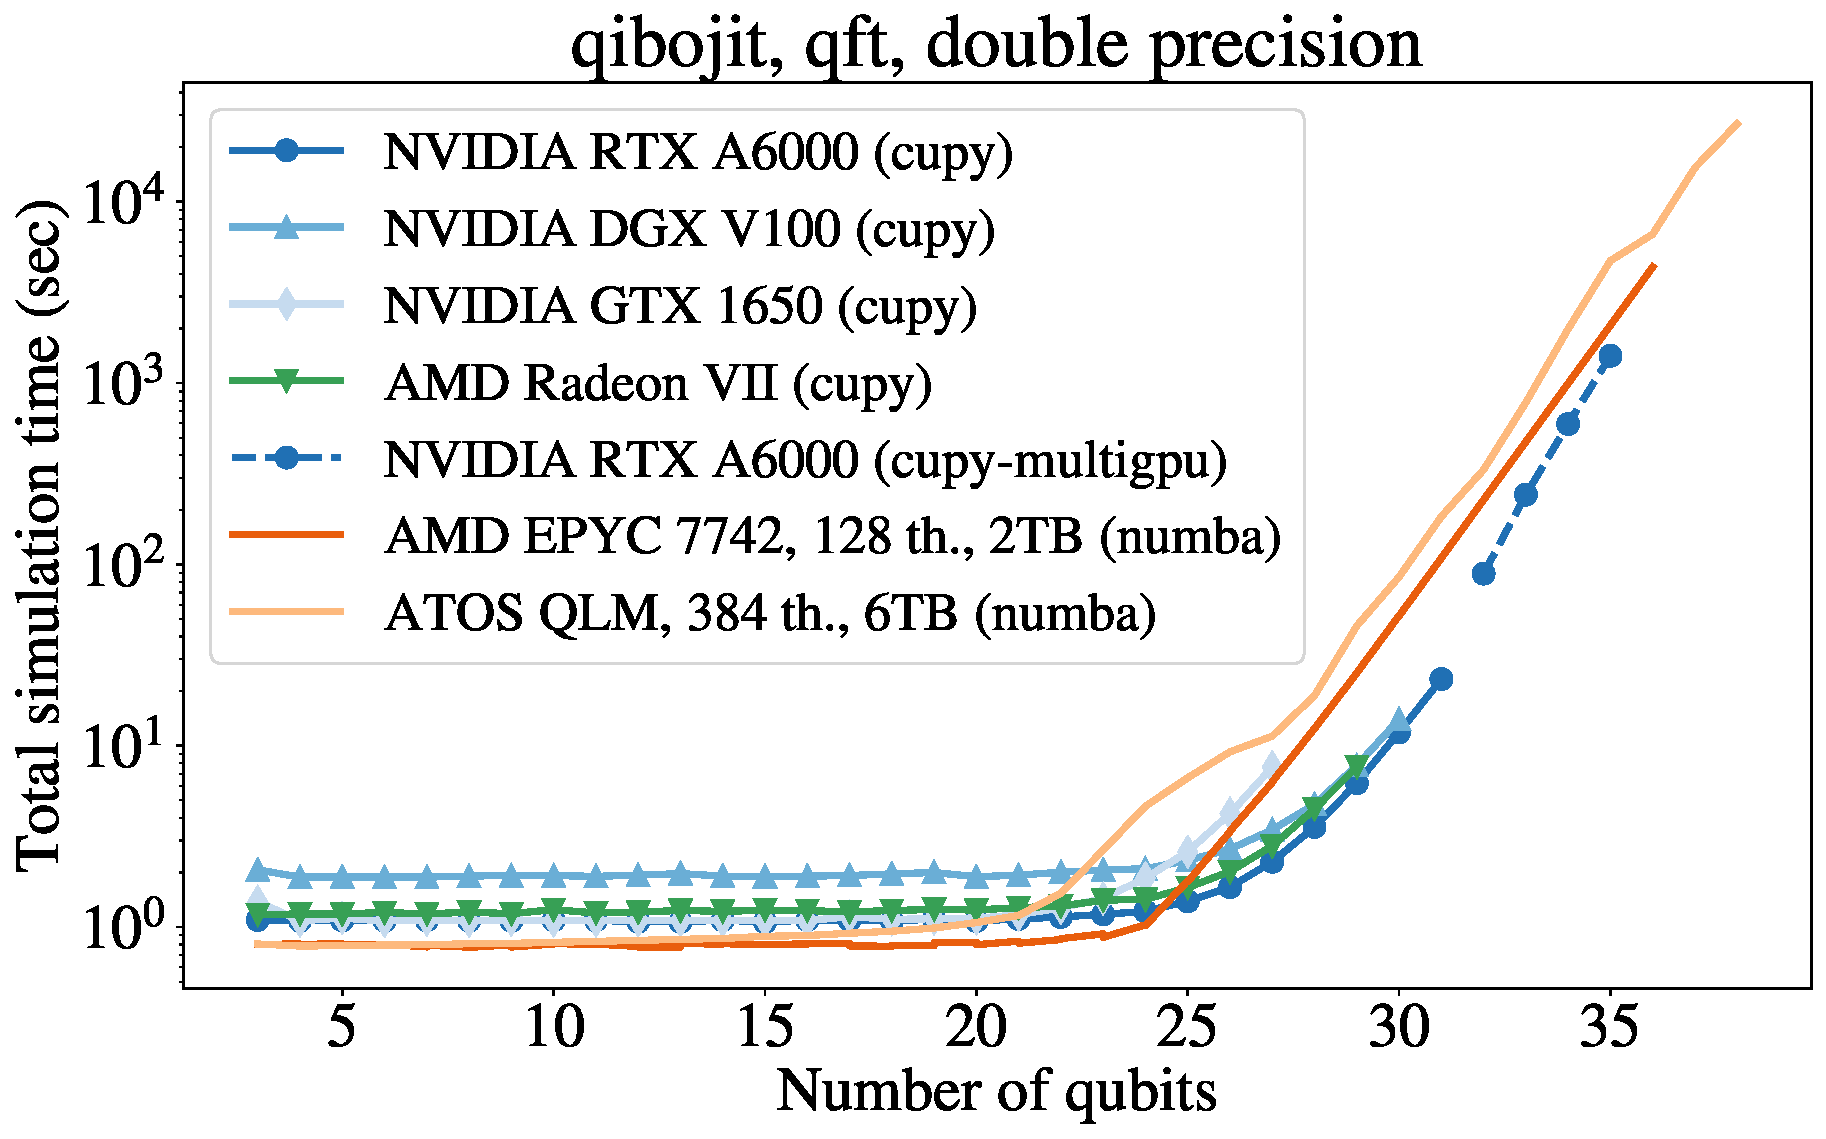
\includegraphics[width=1.\linewidth]{figures/devices_qft_total_simulation_time_double.pdf} 
   \end{figure} 
   \begin{figure}
     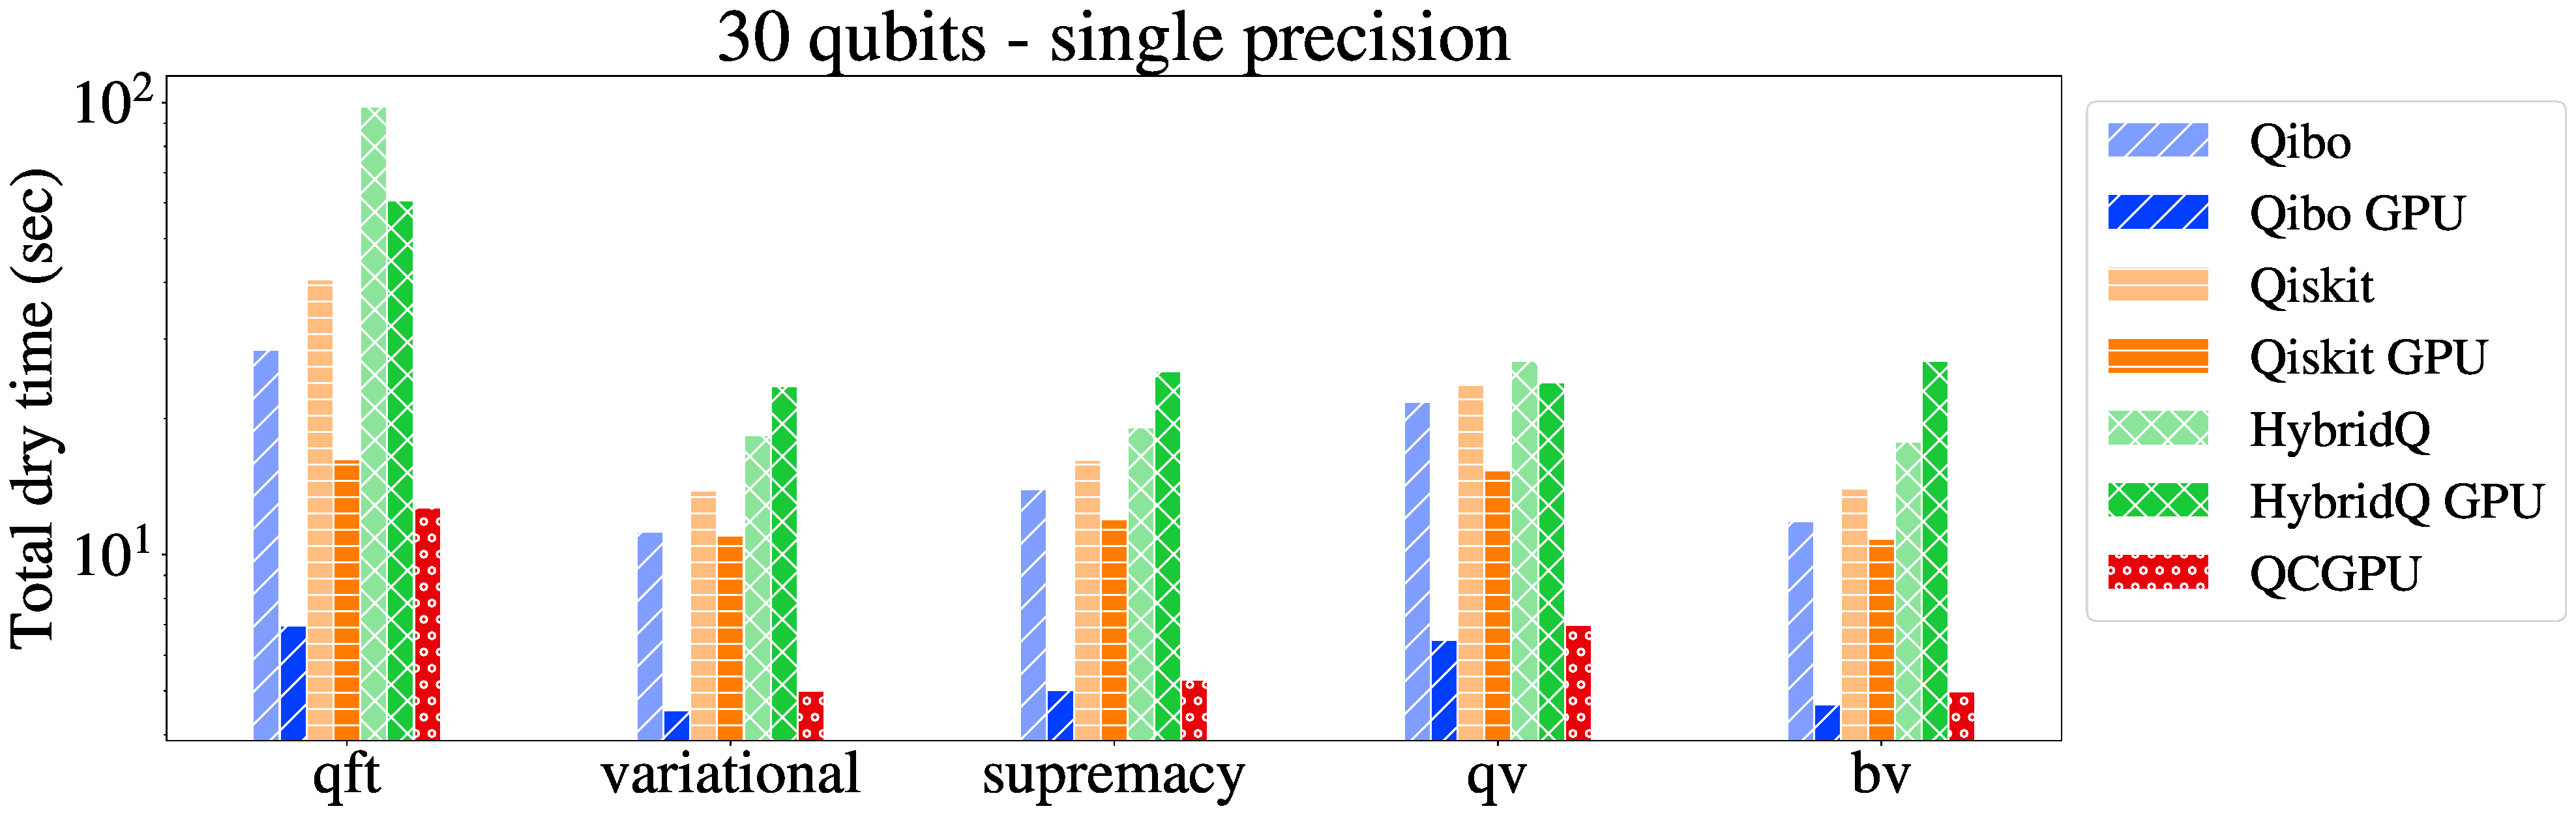
\includegraphics[width=1.\linewidth]{figures/libraries_single_30qubits_total_dry_time.pdf} 
     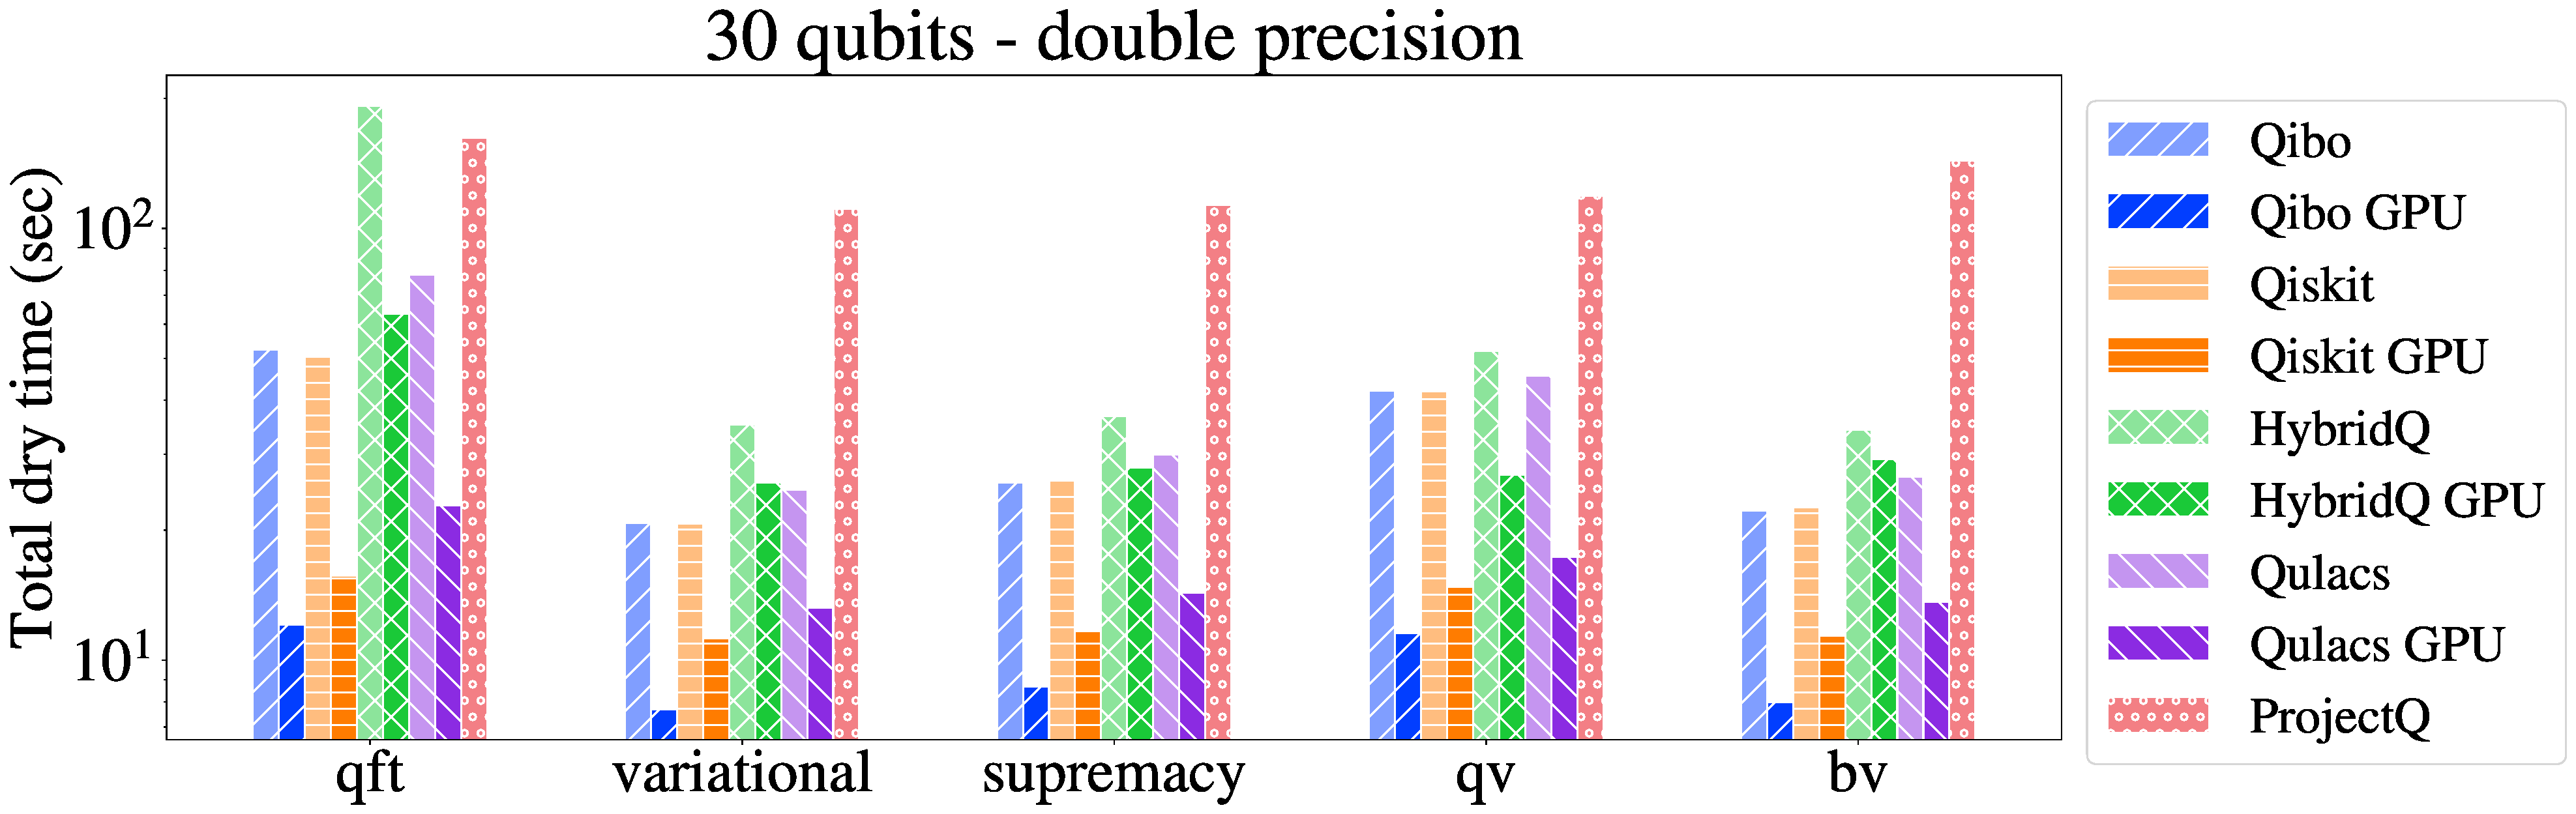
\includegraphics[width=1.\linewidth]{figures/libraries_double_30qubits_total_dry_time.pdf} 
   \end{figure}
\end{multicols}
We reach satisfying performances thanks to custom operators and in-place updates of the statevector.

\end{frame}

\section{Quantum Machine Learning}

\begin{frame}{Classical Machine Learning}
I asked ChatGPT to give me a comprehensive diagram of Machine Learning (ML) models.
\begin{figure}
   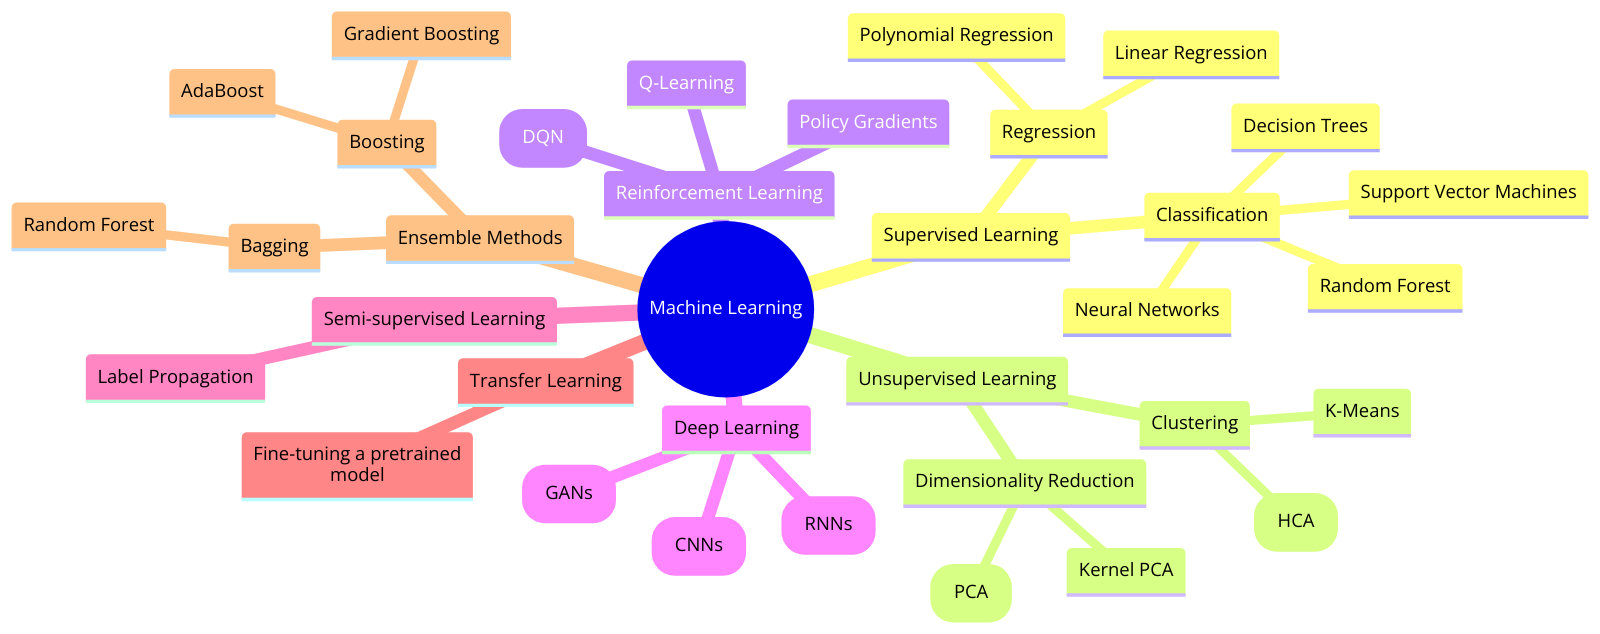
\includegraphics[width=0.7\linewidth, height=0.5\textheight]{figures/ml.png}
\end{figure}  
\textcolor{white}{Focusing on the supervised ML:}
\begin{itemize}[noitemsep]
\item[] \textcolor{white}{we aim to know some hidden law between two variables: $\bm{y}=f(\bm{x})$}
\item[] \textcolor{white}{we define a parameteric model which returns $\bm{y}_{\rm est}=f_{\rm est}(\bm{x}; \bm{\theta})$}
\item[] \textcolor{white}{we define an optimizer, which task is to compute} 
   \textcolor{white}{$\text{argmin}_{\bm{\theta}}\bigl[J(\bm{y}_{\rm meas}, \bm{y}_{\rm est})\bigr]$}
\end{itemize}
\end{frame}

\begin{frame}{Classical Machine Learning}
I asked ChatGPT to give me a comprehensive diagram of Machine Learning (ML) models.
\begin{figure}
   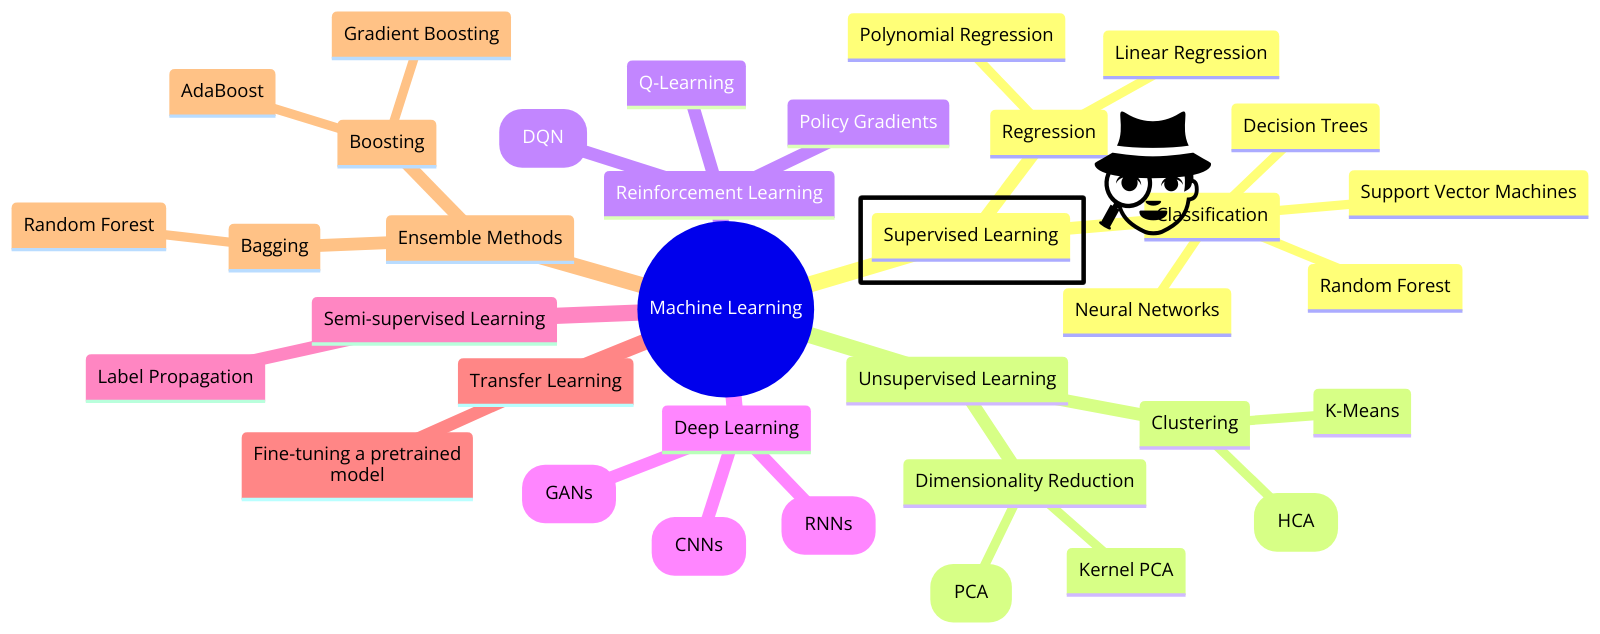
\includegraphics[width=0.7\linewidth, height=0.5\textheight]{figures/supervised.png}
\end{figure}  
Focusing on the supervised ML!
\begin{itemize}[noitemsep]
\item[\faCrosshairs] we aim to know some hidden law between two variables: $\bm{y}=f(\bm{x})$;
\item[\faBarChart] we define a parameteric model which returns $\bm{y}_{\rm est}=f_{\rm est}(\bm{x}; \bm{\theta})$;
\item[\faBinoculars] we define an optimizer, which task is to compute 
   $\text{argmin}_{\bm{\theta}}\bigl[J(\bm{y}_{\rm meas}, \bm{y}_{\rm est})\bigr]$.
\end{itemize}
\end{frame}

\begin{frame}{Classical Machine Learning}
\begin{figure}
   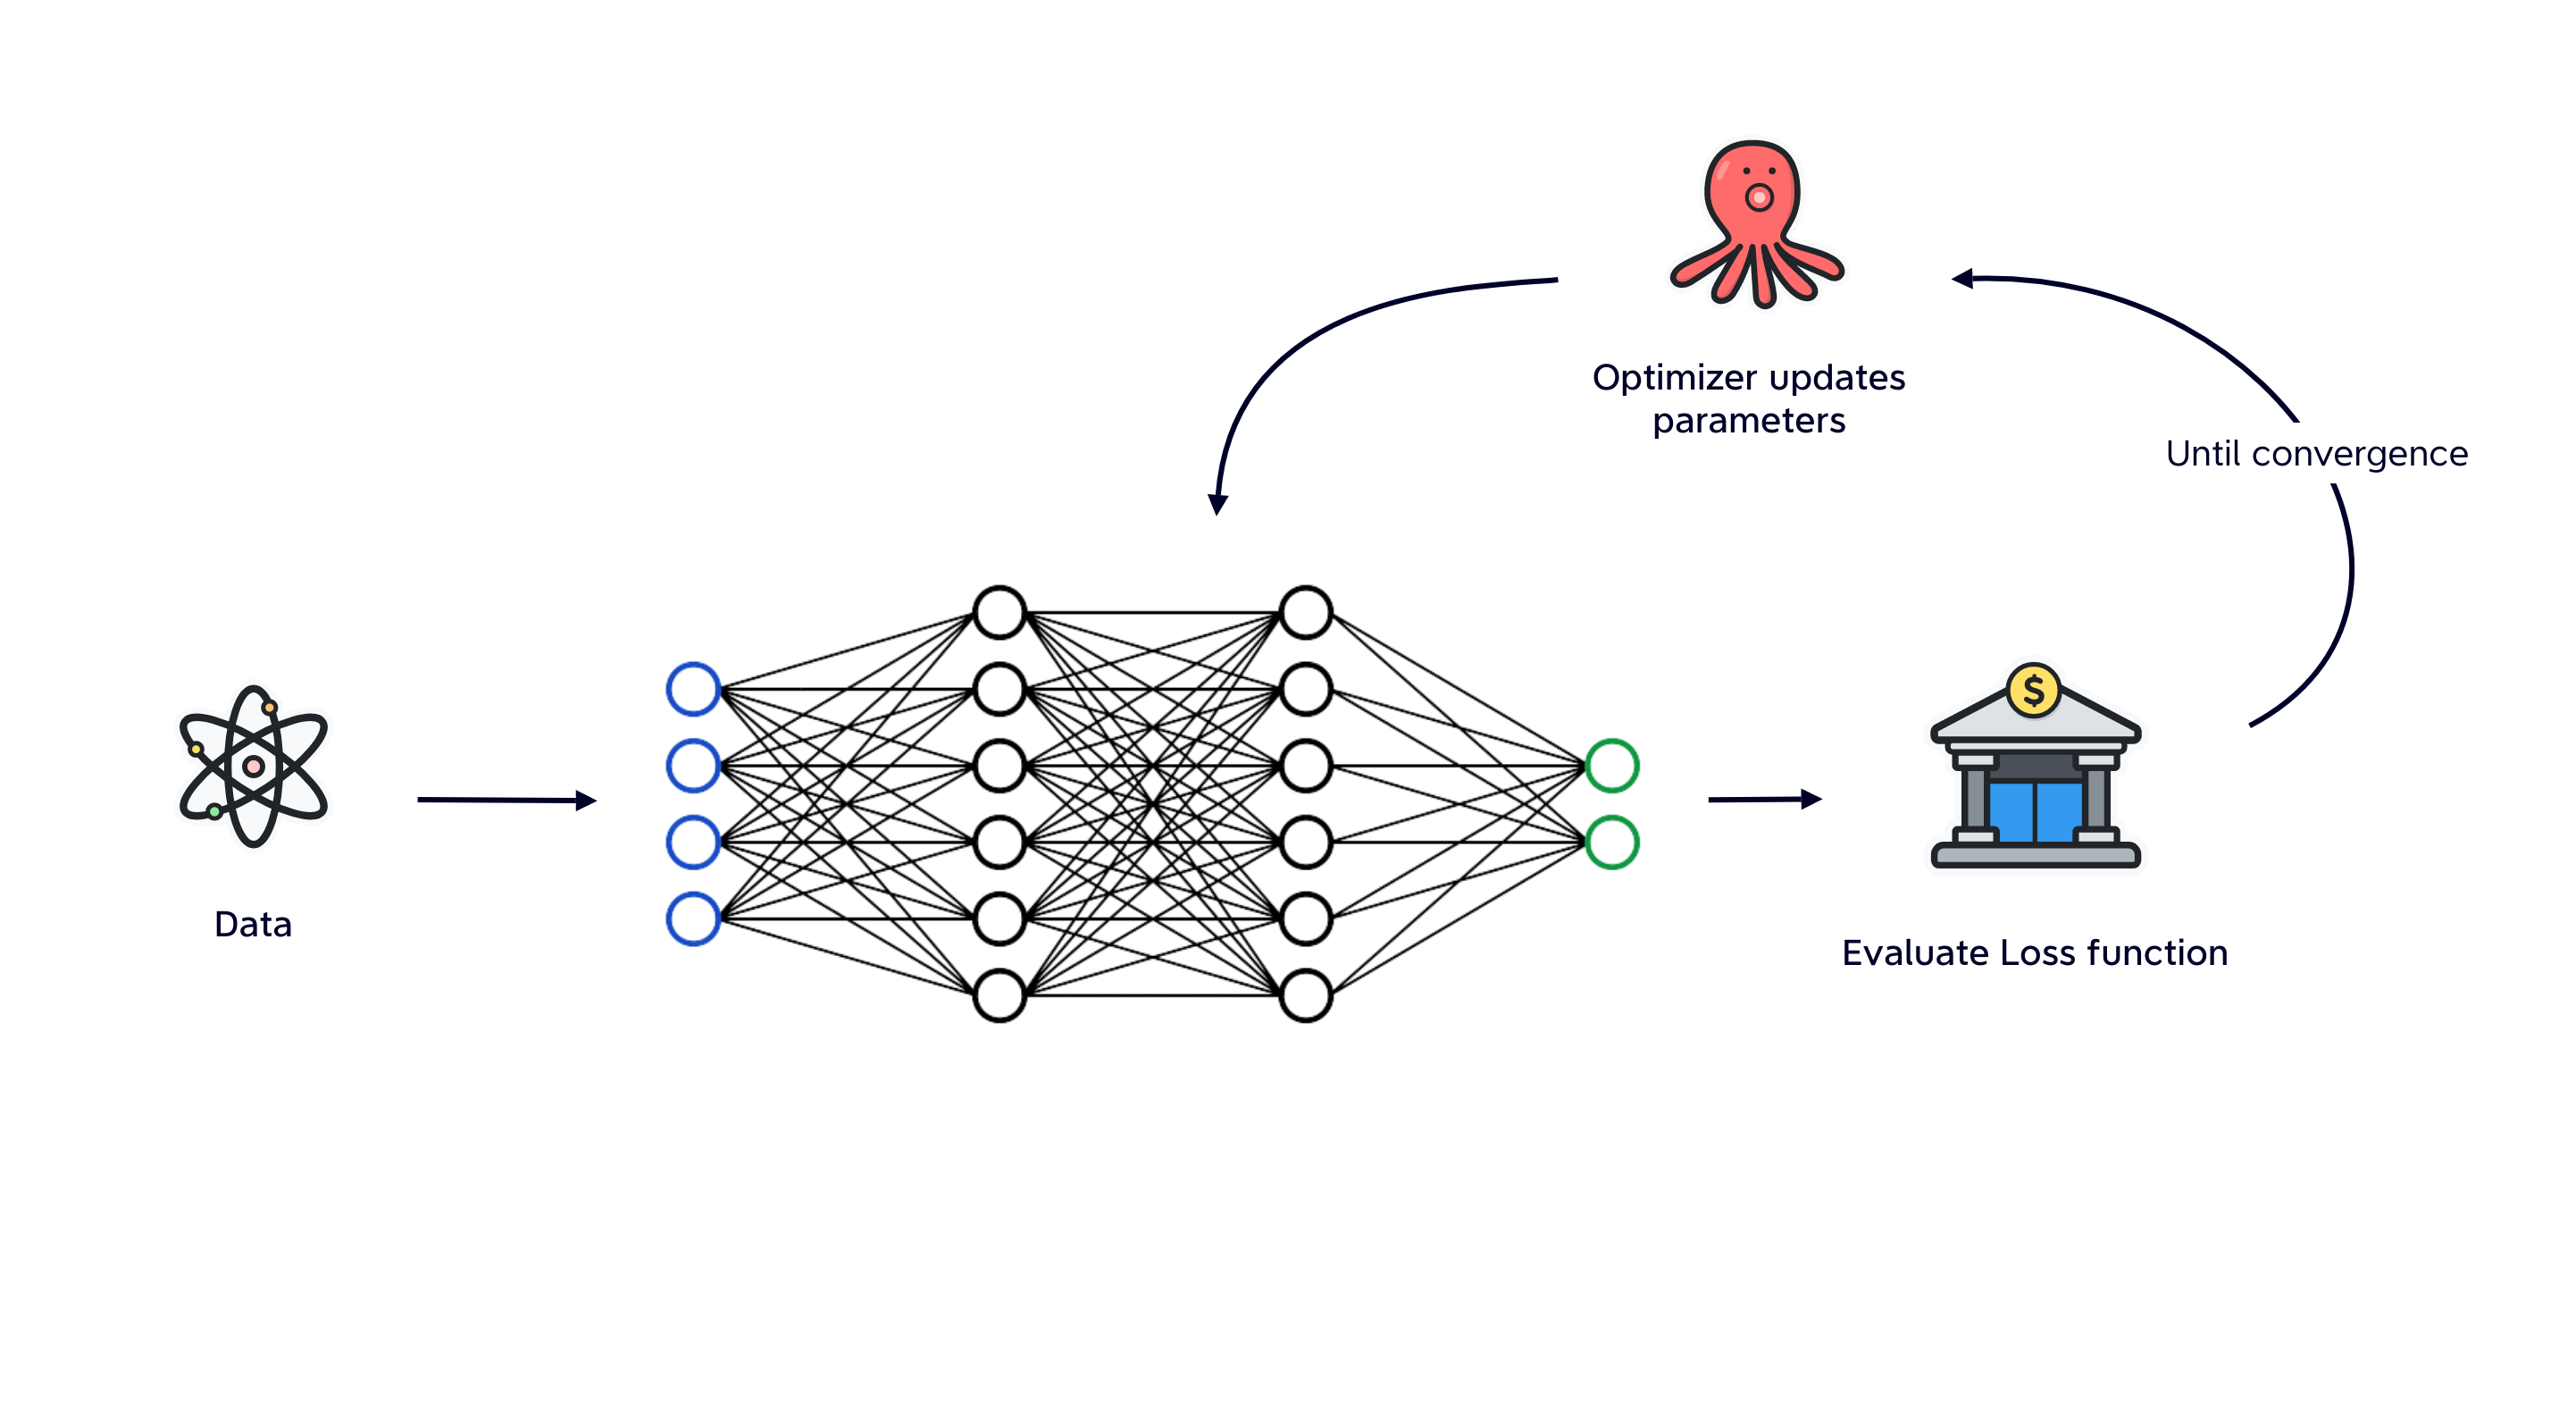
\includegraphics[width=1\linewidth]{figures/ml_scheme.png}
\end{figure}  
\end{frame}



% SLIDE 3 QML
\begin{frame}{Quantum Machine Learning}

\vspace{1.5cm}
\hspace{1cm}    
\begin{tikzpicture}[->,>=stealth']

 \node[state, fill=orange!20] (ML) 
 {\begin{tabular}{l}
 \textbf{Machine Learning}\\ 
 \parbox{2.5cm}{$\mathcal{M}$: model;}\\
 \parbox{2.5cm}{$\mathcal{O}$: optimizer;}\\
 \parbox{2.5cm}{$\mathcal{J}$: loss function.}\\
 \parbox{2.5cm}{$(x, y)$: data}
  \end{tabular}
  };
  
  \node[state,
  below of = ML,
  yshift=-1.5cm, fill=blue!20] (QC) 
 {\begin{tabular}{l}
 \textbf{Quantum Computation}\\ 
 \parbox{2.5cm}{$\mathcal{Q}$: qubits;} \\
 \parbox{2.5cm}{$\mathcal{S}$: superposition;}\\
 \parbox{2.5cm}{$\mathcal{E}$: entanglement.}
  \end{tabular}
  };
  
 \node[state,
    right of=QC,
    yshift=-0.5cm,
    anchor=center,
    node distance=4.5cm, 	
    text width=3.5cm, fill=blue!20] (VQC) 
 {%
 \begin{tabular}{l}
  \textbf{Circuit execution} \\
  \parbox{4.5cm}{
  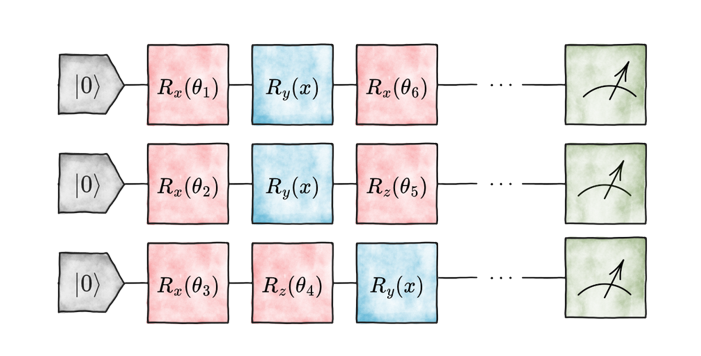
\includegraphics[width=0.9\textwidth]{figures/vqc.png}
  }
 \end{tabular}
 };
 
\node[state,
  right of = VQC,
  node distance = 3cm,
  yshift=2cm, 
  fill=blue!20] (NSHOT) 
 {\begin{tabular}{l}
 \textbf{Expected values}\\ 
 $y_{est} \equiv \braket{q_f|\hat{O}|q_f}$
  \end{tabular}
  };
 
\draw[line width=0.3mm] (1, -2.5)  to[out=0, in=200] (3, -3.2);
\draw[line width=0.3mm] (6, -2.8)  to[out=0, in=250] (7, -1.6);
\end{tikzpicture}

\end{frame}


% SLIDE 4 QML
\begin{frame}{Quantum Machine Learning}

\vspace{0.13cm}
\hspace{1cm}
\begin{tikzpicture}[->,>=stealth']

 \node[state, fill=orange!20] (ML) 
 {\begin{tabular}{l}
 \textbf{Machine Learning}\\ 
 \parbox{2.5cm}{$\mathcal{M}$: model;}\\
 \parbox{2.5cm}{$\mathcal{O}$: optimizer;}\\
 \parbox{2.5cm}{$\mathcal{J}$: loss function.}\\
 \parbox{2.5cm}{$(x, y)$: data}
  \end{tabular}
  };
  
  \node[state,
  below of = ML,
  yshift=-1.5cm, fill=blue!20] (QC) 
 {\begin{tabular}{l}
 \textbf{Quantum Computation}\\ 
 \parbox{2.5cm}{$\mathcal{Q}$: qubits;} \\
 \parbox{2.5cm}{$\mathcal{S}$: superposition;}\\
 \parbox{2.5cm}{$\mathcal{E}$: entanglement.}
  \end{tabular}
  };
  
 
 \node[state,
    right of=QC,
    yshift=-0.5cm,
    anchor=center,
    node distance=4.5cm, 	
    text width=3.5cm, fill=blue!20] (VQC) 
 {%
 \begin{tabular}{l}
  \textbf{Circuit execution} \\
  \parbox{4.5cm}{
  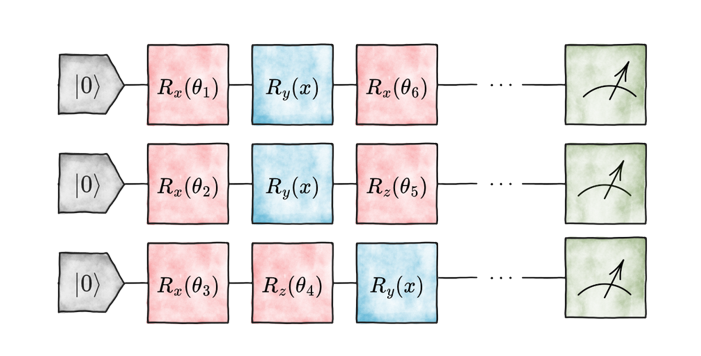
\includegraphics[width=0.9\textwidth]{figures/vqc.png}
  }
 \end{tabular}
 };
 
\node[state,
  right of = VQC,
  node distance = 3cm,
  yshift=2cm, 
  fill=blue!20] (NSHOT) 
 {\begin{tabular}{l}
 \textbf{Expected values}\\ 
 $y_{est} \equiv \braket{q_f|\hat{O}|q_f}$
  \end{tabular}
  };

  
 \draw[line width=0.3mm, red, opacity = 0.7] (0.5, 0.4)  to[out=0, in=230] (3, -3.3);
 \draw[line width=0.3mm, orange, opacity = 0.7] (-1.2, -1.25)  to[out=260, in=300] (4.4, -4.1);
 \draw[line width=0.3mm, cadmiumgreen, opacity = 0.7] (-0.4, -1.2)  to[out=330, in=80] (7.8, -0.4);
  
 
 \draw[red, line width=0.4mm, opacity = 0.9] (-1.1, 0.4) circle (0.4 cm);
 \draw[cadmiumgreen, line width=0.4mm, opacity = 0.9] (-0.65,-0.8) circle (0.3 cm);
 \draw[cadmiumgreen, line width=0.4mm, opacity = 0.9] (7.2,-1.4) rectangle (8.6, -0.95);
 \draw[orange, line width=0.4mm, opacity = 0.6] (-1.15,-0.8) circle (0.3 cm);
 \draw[red, line width=0.4mm, opacity = 0.6] (3.1,-4) rectangle (6,-2.4);
 \draw[orange, line width=0.4mm, opacity = 0.9] (3.5,-3.9) rectangle (5.2,-2.5);


\end{tikzpicture}
\end{frame}


% SLIDE 5 QML
\begin{frame}{Quantum Machine Learning!}
\vspace{-0.01cm}
\hspace{1cm}
\begin{tikzpicture}[->,>=stealth']

 \node[state, fill=orange!20] (ML) 
 {\begin{tabular}{l}
 \textbf{Machine Learning}\\ 
 \parbox{2.5cm}{$\mathcal{M}$: model;}\\
 \parbox{2.5cm}{$\mathcal{O}$: optimizer;}\\
 \parbox{2.5cm}{$\mathcal{J}$: loss function.}\\
 \parbox{2.5cm}{$(x, y)$: data}
  \end{tabular}
  };
  
  \node[state,
  below of = ML,
  yshift=-1.5cm, fill=blue!20] (QC) 
 {\begin{tabular}{l}
 \textbf{Quantum Computation}\\ 
 \parbox{2.5cm}{$\mathcal{Q}$: qubits;} \\
 \parbox{2.5cm}{$\mathcal{S}$: superposition;}\\
 \parbox{2.5cm}{$\mathcal{E}$: entanglement.}
  \end{tabular}
  };
  

 \node[state,   
  text width=3cm, 
  yshift=1.5cm, 
  right of=ML, 	
  node distance=4cm, 
  anchor=center, fill=green!20] (OPT) 
 {%
 \begin{tabular}{l} 	% content
  \textbf{Optimizer $\mathcal{O}$}\\
  Hybrid-strategy
 \end{tabular}
 };
 
 \node[state,
    right of=QC,
    yshift=-0.5cm,
    anchor=center,
    node distance=4.5cm, 	
    text width=3.5cm, fill=blue!20] (VQC) 
 {%
 \begin{tabular}{l}
  \textbf{Circuit execution} \\
  \parbox{4.5cm}{
  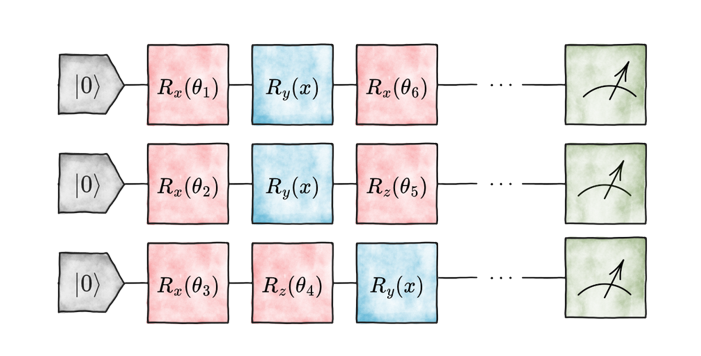
\includegraphics[width=0.9\textwidth]{figures/vqc.png}
  }
 \end{tabular}
 };
 
\node[state,
  right of = VQC,
  node distance = 3cm,
  yshift=2cm, 
  fill=blue!20] (NSHOT) 
 {\begin{tabular}{l}
 \textbf{Expected values}\\ 
 $y_{est} \equiv \braket{q_f|\hat{O}|q_f}$
  \end{tabular}
  };
  
  \node[state,
  above of = NSHOT,
  node distance = 1.5cm,
  yshift=0cm, fill=green!20] (J) 
 {\begin{tabular}{l}
 \textbf{loss function $\mathcal{J}$}\\ 
 $\mathcal{J}(y_{meas}, y_{est})$
  \end{tabular}
  };
  

 \draw[line width=0.3mm] (6.5, -3)  to[out=0, in=270] (7.5, -1.6);
 \draw[line width=0.3mm] (6, -1.1)  to[out=180, in=200] (6.1, 0.2);
 \draw[line width=0.3mm] (7.5, 1.1)  to[out=90, in=0] (5.7, 1.5);
 \draw[line width=0.6mm, opacity=0.8] (2, 1.6)  to[out=180, in=270] (-0.2, 2.9);
 
 \draw[line width=0.3mm, orange, opacity = 0.0] (-1.2, -1.25)  to[out=260, in=300] (4.4, -3.5);

\end{tikzpicture}
\end{frame}

\begin{frame}{From ML to QML}
\begin{figure}  
   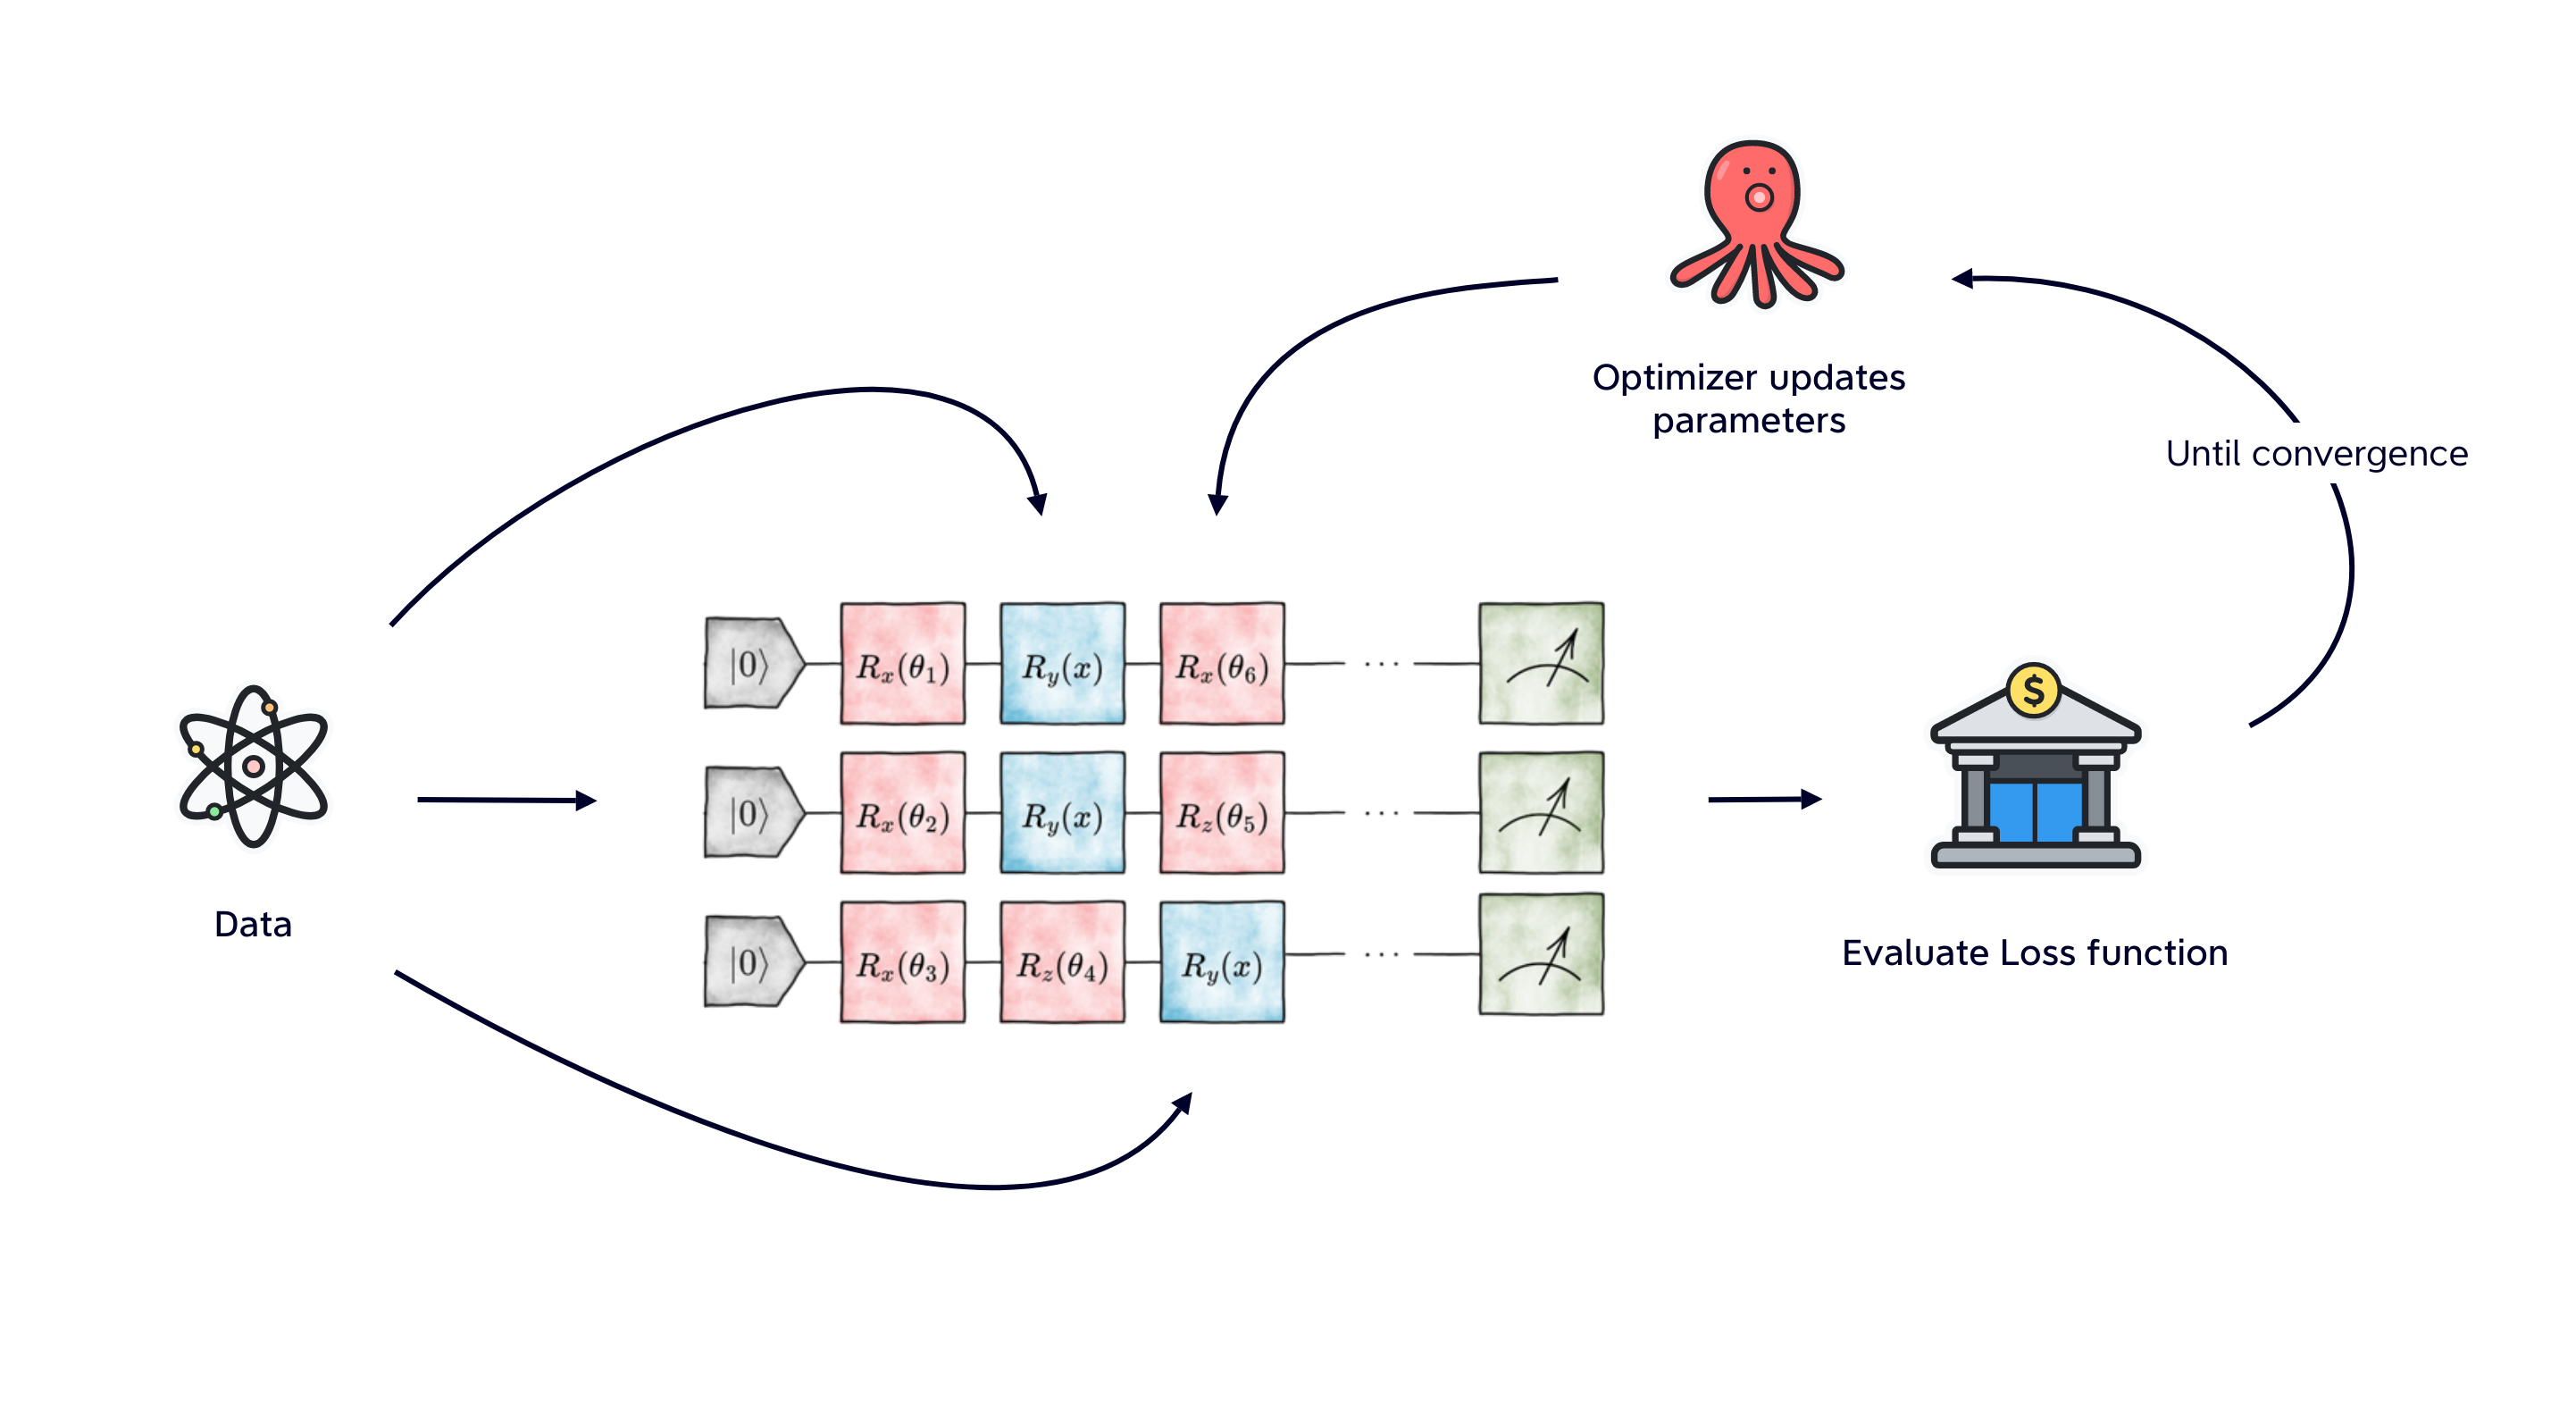
\includegraphics[width=1\textwidth]{figures/qml_scheme.png}
\end{figure}
\end{frame}

\begin{frame}[fragile]{Example 2: PDF fit \hfill \faBook\,\, \href{https://arxiv.org/abs/2011.13934}{arXiv:2011.13934}}

  \small
  We parametrize \textbf{Parton Distribution Functions} with multi-qubit variational quantum circuits:
  \begin{columns}
    \column{6cm}
    \begin{itemize}
      \item[1.] Define a quantum circuit: $\mathcal{U}(\theta, x) | 0 \rangle ^ {\otimes n} = | \psi (\theta, x) \rangle$
      \item[2.] $U_w (\alpha, x) = R_z(\alpha_3 \log(x) + \alpha_4) R_y(\alpha_1 \log(x) + \alpha_2)$
      \item[3.] Using $z_i (\theta, x) = \langle \psi (\theta, x) | Z_i | \psi (\theta, x) \rangle$:
      \begin{equation*}
        {\rm qPDF}_i (x, Q_0, \theta) = \frac{1-z_i (\theta, x)}{1+z_i(\theta, x)}.
      \end{equation*}
    \end{itemize}

    \column{4cm}
    \vspace{-0.2cm}
    \begin{figure}
      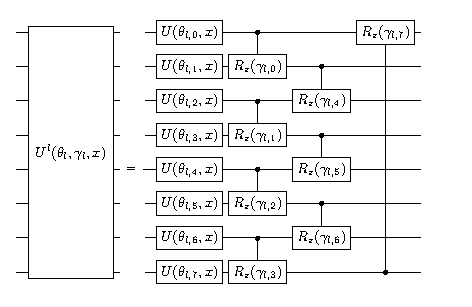
\includegraphics[height=3cm]{figures/layer.pdf}
    \end{figure}
  \end{columns}

  Results from \textbf{\color{teal} classical quantum simulation and hardware execution} (IBM) are \textbf{promising}:
  \begin{figure}
    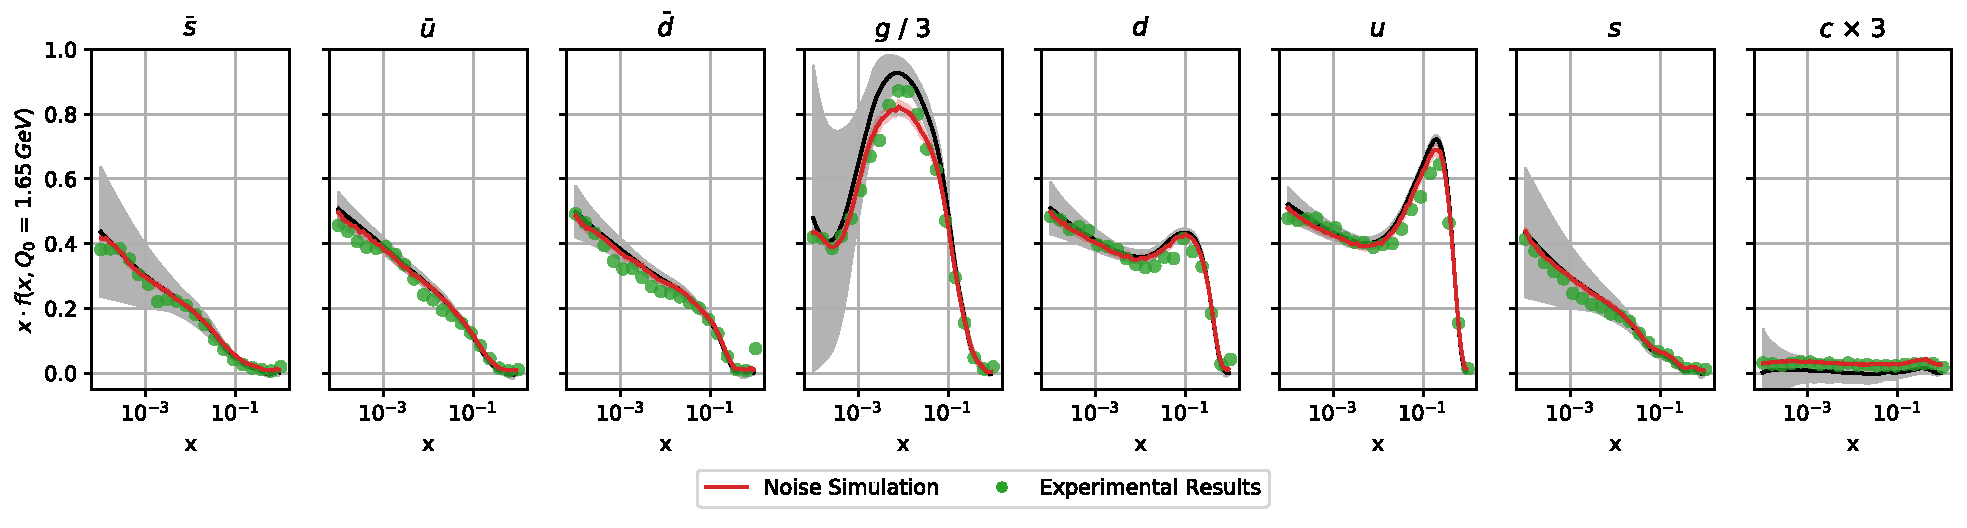
\includegraphics[width=0.9\textwidth]{figures/Experiments-SingleFlavor.pdf}
  \end{figure}

\end{frame}


\begin{frame}{PDF fit on chip \hfill \faBook\,\, \href{https://arxiv.org/abs/2308.06313}{arXiv:2308.06313}}

\begin{multicols}{2}
% column 1
\hspace{2cm}
\begin{tcolorbox}[title=High level API: Qibo, colback=blue!20]
\begin{itemize}[noitemsep]
\small
   \item[\faCode] define \textbf{prototypes} and models;
   \item[\faCode] \textbf{simulate} training and noise.
\end{itemize}
\end{tcolorbox}
\begin{tcolorbox}[title=Calibration: Qibocal, colback=yellow!20]
\begin{itemize}[noitemsep]
\small
   \item[\faCrosshairs] \textbf{calibrate} qubits;
   \item[\faCrosshairs] generate \textbf{platform configuration};
\end{itemize}
\end{tcolorbox}
\begin{tcolorbox}[title=Execution: Qibolab, colback=red!20]
\begin{itemize}[noitemsep]
\small
   \item[\faCog] allocate \textbf{calibrated} platform;
   \item[\faCog] \textbf{compile} and \textbf{transpile} circuits;
   \item[\faCog] execute and return \textbf{results}.
\end{itemize}
\end{tcolorbox}
% column 2
% PDF image
\begin{figure}  
    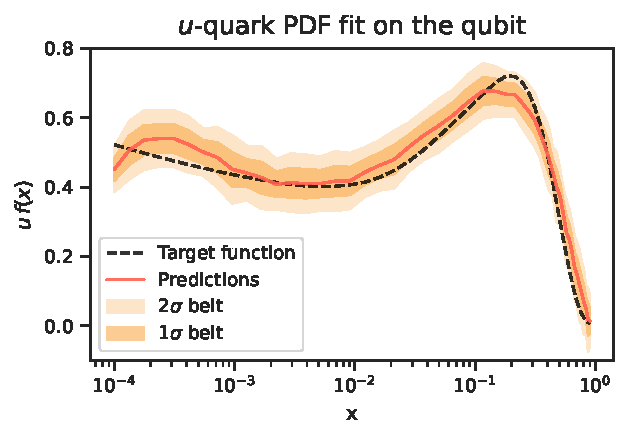
\includegraphics[width=0.38\textwidth]{figures/qpdf.pdf}
\end{figure}
% parameters
\begin{center}
\begin{table}
\vspace{-0.5cm}
\begin{tabular}{cc}
\hline \hline 
\textbf{Parameter} & \textbf{Value} \\
\hline 
$N_{\rm data}$ & 50 \\
$N_{\rm shots}$ & 500 \\
MSE & $\sim 10^{-3}$ \\
Electronics & Xilinx ZCU216 \\
Training time & $\sim 2$h \\
\hline \hline
\end{tabular}
\end{table}
\end{center}
\vspace{0.5cm}
\end{multicols}
\begin{picture}(0,0)
    \put(355,75){
        
\includegraphics[width=0.12\textwidth]{figures/homemade.png}
    }
\end{picture}
\end{frame}

\begin{frame}{Some applications}
  \small
  %\only<2-3>{\vspace{0.1cm}}
  \begin{itemize}
  \item[-] Multi-variable integration using the qPDF ansatz, \href{https://arxiv.org/abs/2303.11346}{\faBook\,\,arXiv:2303.11346};
  \item[-] Real-time quantum error mitigation on superconducting devices to improve trainability,
  \href{https://arxiv.org/abs/2303.11346}{\faBook\,\,arXiv:2303.11346};
  \end{itemize}
    \begin{figure}
      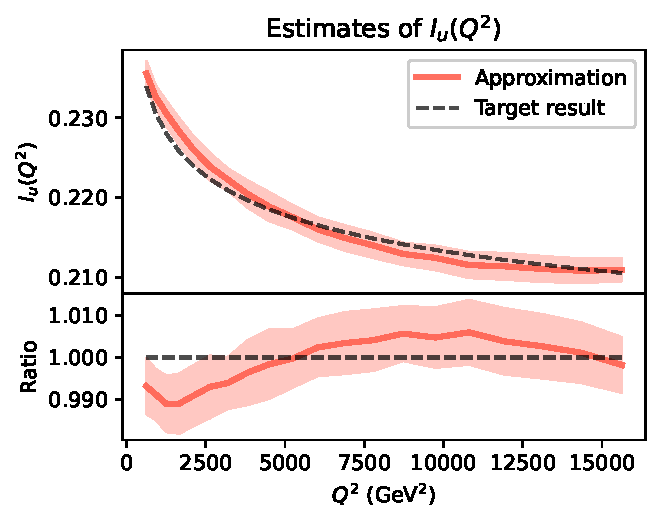
\includegraphics[width=0.45\textwidth]{figures/uquark2d.pdf}%
      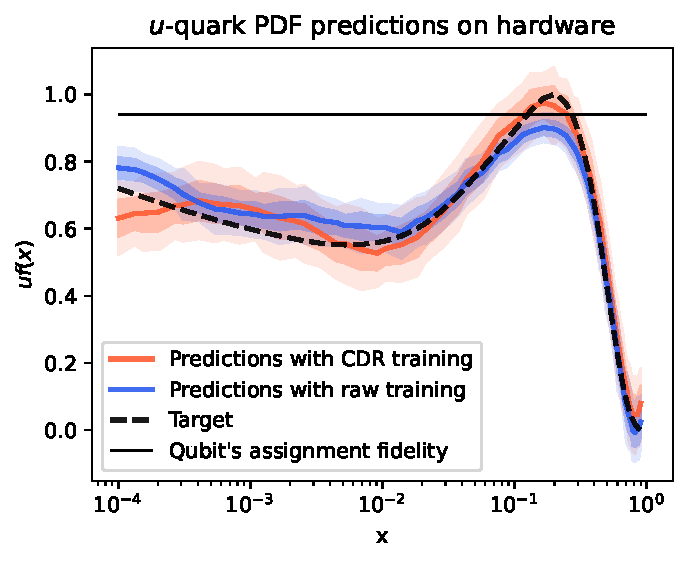
\includegraphics[width=0.45\textwidth]{figures/hardware.pdf}
    \end{figure}
\end{frame}

\end{document}
